\documentclass[phd,tocprelim]{cornell}

%
% tocprelim option must be included to put the roman numeral pages in the
% table of contents
%
% The cornellheadings option will make headings completely consistent with
% guidelines.
%
% This sample document was originally provided by Blake Jacquot, and
% fixed up by Andrew Myers.
%
%Some possible packages to include
\usepackage{amsmath}
\usepackage{graphicx,pstricks}
\usepackage{graphics}
\usepackage{moreverb}
\usepackage{subfigure}
\usepackage{epsfig}
\usepackage{subfigure}
\usepackage{hangcaption}
\usepackage{txfonts}
\usepackage{listings}
\usepackage{palatino}
\usepackage{algorithm}
\usepackage{multirow}
\usepackage{url}
\usepackage{bm}
% \usepackage{siunitx}
\usepackage{xspace}

\usepackage{algcompatible}
\usepackage[floatrow]{trivfloat}
\trivfloat{algorithm}
\renewcommand\algorithmname{ALGORITHM}

\let\oldAA\AA
\renewcommand{\AA}{\text{\normalfont\oldAA}}

\newcommand\nd{\textsuperscript{nd}\xspace}
\newcommand\rd{\textsuperscript{rd}\xspace}
\newcommand\nth{\textsuperscript{th}\xspace} %\th is taken already

\lstset{basicstyle=\small\ttfamily,breaklines=true}
% \usepackage{ctex}

%if you're having problems with overfull boxes, you may need to increase
%the tolerance to 9999
\tolerance=9999

\bibliographystyle{plain}
%\bibliographystyle{IEEEbib}

\renewcommand{\caption}[1]{\singlespacing\hangcaption{#1}\normalspacing}
\renewcommand{\topfraction}{0.85}
\renewcommand{\textfraction}{0.1}
\renewcommand{\floatpagefraction}{0.75}

\title {Fast Semistochastic Heat-Bath Configuration Interaction}
\author {Junhao Li}
\conferraldate {June}{2019}
\degreefield {Ph.D.}
\copyrightholder{Junhao Li}
\copyrightyear{2019}

\begin{document}

\maketitle
\makecopyright

\begin{abstract}
In this thesis, I present my work on the fast semistochastic heat-bath configuration interaction, which is an efficient algorithm for solving the many-body solving electronic structure calculations and computational research on large clusters. Arrow provides two sets of features: a quantum solver based on the Fast Semistochastic Heatbath Configuration Interaction (Fast SHCI) algorithm recently developed in our group, and several generic distributed computing building blocks.

Fast SHCI [Junhao Li et al., JCP 2018] is more than 100 times faster than other algorithms in its category (selected CI plus perturbation theory), and also much faster than other essentially exact algorithms for most chemical systems. This thesis provides an in-depth description of the Fast SHCI algorithm and its implementation in Arrow. I use Arrow to compute electronic structures of several chemical systems and the homogeneous electron gas.  Some of these calculations are more accurate than those achieved by other high-order quantum chemistry methods.  Others treat systems larger than those that can be treated by other equally accurate methods.

Arrow uses a modular design, which not only makes the library highly extensible but also contributes several generic distributed computing building blocks to the open-source community. The high-level components that come with Arrow include:
(1) A data serialization library that is upto four times faster and produces more compact serialized messages than widely used libraries in industry;
(2) A highly optimized cluster computing library that is upto eight times faster than Apache Spark on common data processing tasks;
(3) A modified version of Google Test for testing distributed computing modules.
In this thesis, I discuss my design and implementation of all of them.

Finally, I also provide a brief discussion of the usability of general software engineering best practices for the development of medium-scale scientific software packages with lessons learned from designing, developing, and leading the development of Arrow. Medium-scale scientific software packages are common in scientific research where a small group of researchers works on the same code base. Due to the differences in the requirements, some best practices that are common in industry need to be adjusted to be useful for these projects.

Your abstract goes here. Make sure it sits inside the brackets. If not,
your biosketch page may not be roman numeral iii, as required by the
graduate school.
\end{abstract}

\begin{biosketch}
Junhao Li was born and grew up in Shanghai, China.
From a young age, he had a strong interest in science and engineering, and enjoyed disassembling all kinds of home appliances.

Junhao attended Shanghai Jiao Tong University from 2009, graduating with a B.S. in physics and a B.S.E in computer science in 2013.
While an undergraduate, he did research in various fields, including semiconductor fabrication, photovoltaics, finite element analysis of electromagnetic field, density functional theory, and social networks.

In the fall of 2013, Junhao came to Cornell University to persue a Ph.D. in physics.
During his Ph.D, he mainly worked with professor Cyrus Umrigar on the development and application of highly accurate quantum chemistry methods.
He developed the fast heat-bath configuration interaction method, which is faster than other methods in its category by more than an order of magnitude, and achieved significantly higher accuracy than other well developed methods, such as DMRG and FCIQMC, on several systems.
he also did research in molecular dynamics and defects with professor James Sethna.

After obtaining a master's degree at Cornell, Junhao spent a summer as an intern at Google in California in 2016.
He then returned to Ithaca, brought back the engineering merits he learned from Google, and developed a highly efficient and extensible quantum chemistry package, Arrow, as well as several open-sourced generic high performance computing libraries.
\end{biosketch}

\begin{dedication}
This document is dedicated to all Cornell graduate students.
\end{dedication}

\begin{acknowledgements}
First of all, I would like to thank my advisor Professor Cyrus Umrigar.
His commitment to physics research is exemplary and inspiring.
He led me into the field of quantum chemistry, which is an indispensable foundation of highly accurate numerical simulations.
All my knowledge of quantum Monte Carlo are inherited from him, and my work on heat-bath configuration interaction is impossible without his guidance and support.
He also taught me valuable research skills, and helped me go through the process of publishing my first first-author paper, on a top academic journal.
I am also extremely grateful to him for always being supportive in the decisions I made, the ideas I wanted to try, and being tolerant and direct with the mistakes I made.
He made my six years of Ph.D life a truly rewarding experience.

I would also like to thank Professor James Sethna.
It was a pleasure to work with Jim on defects and molecular dynamics.
His enthusiasm and optimism inspires me whenever I face chanllenging problems.
I also learned a lot from his tremendous physics and data insights.

I also thank all the graduate students I worked with, especially Adam Holms, Matt Otten, and Matt Bierbaum.
They helped me getting started in my research, patiently answered all my questions, and gave me valuable advices on my projects.
I could not imagine how much longer it would take me to get start and how many detours I might have taken without their help.

Special thanks to my parents for giving me birth and raising me up.
They gave me a warm family as I grew up, and consistently support as I persue my degree at Cornell.
Thanks also to my elementary school, middle school, high school, and undergraduate teachers and friends back in China for all the invaluable lessons I learned from them, the wonderful memories I had with them, and helps and encouragements I received from them.

Finally, I acknowledge the financial support from the Cornell physics department, National Science Foundation and the Air Force Office of Scientific Research, and the computing resources support from Pittsburg Computing Center, Argonne National Lab, NERSC, and Google Cloud.
Thank you and I hope you are proud.
\end{acknowledgements}

\contentspage
\tablelistpage
\figurelistpage

\normalspacing \setcounter{page}{1} \pagenumbering{arabic}
\pagestyle{cornell} \addtolength{\parskip}{0.5\baselineskip}

\chapter{Introduction}


\def\beq{\begin{eqnarray}}
\def\eeq{\end{eqnarray}}
\def\V{\mathcal{V}}
\def\C{\mathcal{C}}
\def\P{\mathcal{P}}

\def\NMCdiff{{N_{\mathrm{MC}}^{\mathrm{uniq}}}}
\def\Nd{{N_d}}
\def\Nddiff{{N_{d}^{\mathrm{uniq}}}}

\def\vecD{\vec{D}}
\def\veca{\vec{\alpha}}
\def\vecb{\vec{\beta}}
\def\ia{i_\alpha}
\def\ja{j_\alpha}
\def\ib{i_\beta}
\def\veciD{\vec{i}_D}
\def\vecia{\vec{i}_\alpha}
\def\vecib{\vec{i}_\beta}
\def\veciDa{\vec{i}_{D\alpha}}
\def\veciDb{\vec{i}_{D\beta}}
\def\veciaa{\vec{i}_{\alpha\alpha}}
\def\veciba{\vec{i}_{\beta\alpha}}
\def\veciab{\vec{i}_{\alpha\beta}}
\def\vecibb{\vec{i}_{\beta\beta}}

\chapter{Fast Heat-Bath Configuration Interaction}
This chapter presents in detail our fast semistochastic heat-bath configuration interaction (SHCI) method for solving the many-body Schr\"{o}dinger equation.
We identify and eliminate computational bottlenecks in both the variational and perturbative steps of the SHCI algorithm.
We also describe the parallelization and the key data structures in our implementation, such as the distributed hash table.
% To achieve high computational efficiency for large systems, we use distributed hash tables.
%The improved SHCI is blazing fast.
The improved SHCI algorithm enables us to include in our variational wavefunction two orders of magnitude more determinants
than has been reported previously with other selected configuration interaction methods.

\section{Introduction}
The choice of quantum chemistry methods requires a trade-off between accuracy and efficiency.
Density functional theory
%(DFT)~\cite{parr1979local,perdew1996generalized,kohn1999nobel}
(DFT)~\cite{ParYan-BOOK-89,DreGro-BOOK-90,kohn1999nobel}
methods with approximate density functionals
are popular and efficient, but are often not sufficiently accurate.  Coupled cluster with single, double, and perturbative triple excitations CCSD(T)~\cite{raghavachari1989fifth} is very accurate for single reference systems, but
not for strongly-correlated systems, such as systems with stretched bonds.
Density matrix renormalization group (DMRG)~\cite{white1993density,white1999ab,chan2002highly,chan2011density,ShaCha-JCP-12,olivares2015ab,schollwock2005density,GuoLiCha-JCTC-18}
and full configuration interaction quantum Monte Carlo (FCIQMC)~\cite{BooThoAla-JCP-09,CleBooAla-JCP-10,PetHolChaNigUmr-PRL-12,BooGruKreAla-Nat-13,HolChaUmr-JCTC-16}
are systematically improvable but rapidly get expensive with the number of electrons and the size of the basis set.

The recently developed semistochastic heat-bath configuration interaction (SHCI)~\cite{HolTubUmr-JCTC-16,ShaHolJeaAlaUmr-JCTC-17,HolUmrSha-JCP-17,SmiMusHolSha-JCTC-17,MusSha-JCTC-17,ChiHolOttUmrShaZim-JPCA-18} is another systematically improvable method capable of providing essentially exact energies for small systems.
In common with FCIQMC, the computational cost of the method scales exponentially in the number of electrons but with a
much smaller exponent than in full configuration interation (FCI).  However, SHCI is much faster than FCIQMC.
The comparison with DMRG is more involved.
%SHCI is often much faster than DMRG for moderately correlated systems,
%however, is much less efficient than DMRG for quasi 1-dimensional systems and even some strongly correlated 
%higher-dimensional spin systems. %{\color{red} which? Sandeep wanted to leave this a bit vague because it is not completely clear.}
{\color{black}
While SHCI is much faster than DMRG for small moderately correlated systems, the ratio of costs changes in
DMRG's favor as the system size increases and as the correlation strength increases, because the methods
have different scaling with these parameters.
%In particular SHCI scales exponentially with system size with a small prefactor, with the prefactor depending on
In particular SHCI scales exponentially with system size with a prefactor that is typically small, but which grows with
the strength of the correlation.
DMRG scales exponentially with the $(D-1)/D$-th power of the system size (where D is the system dimension) with a prefactor that is typically larger,
but is not very sensitive to the strength of the correlation.
}

SHCI is an example of the selected configuration interaction plus perturbation theory (SCI+PT)
methods~\cite{HurMalRan-JCP-73,BuePey-TCA-74,EvaDauMal-CP-83,CimPer-JCoP-87,Har-JCP-91,BytRue-CP-09,KelPerBarGre-JCP-14,CoeMurPat-CPL-14,Eva-JCP-14,SceAppGinCaf-JCoC-16,GarSceLooCaf-JCP-17,LooSceBloGarCafJac-JCP-18,TubLevHaiHeaWha-ARX-18},
the earliest of which being
the configuration interaction by perturbatively selecting iteratively (CIPSI) method~\cite{HurMalRan-JCP-73,EvaDauMal-CP-83} of Malrieu and collaborators.
SCI+PT methods have two stages.  In the first stage a variational wavefunction is constructed iteratively, starting from
%the Hartree-Fock determinant, or more generally a determinant
a determinant that is expected to have a significant amplitude in the final wavefunction, e.g., the Hartree-Fock determinant.
Each iteration of the variational stage has three steps: selection of important determinants, construction of the Hamiltonian matrix, and
iterative diagonalization of the Hamiltonian matrix.
In the second stage, 2$^{\rm nd}$-order perturbation theory is used to improve upon the variational energy.

The SHCI algorithm has greatly improved the efficiency of both stages.
First, as discussed in Section~\ref{Var}, it greatly speeds up the determinant selection, and, second, as discussed in
Section~\ref{PT}, it drastically reduces the central processing unit (CPU) cost as well as the memory cost of performing the perturbation step by using a semistochastic algorithm.
These two modifications have allowed SHCI to be used for systems as large as hexatriene
in an ANO-L-pVDZ basis (32 correlated electrons in 118 orbitals) which has a Hilbert space of $10^{38}$ determinants~\cite{ChiHolOttUmrShaZim-JPCA-18}.
SHCI has also recently been extended to (a) calculate not just the ground state but also the low-lying excited states~\cite{HolUmrSha-JCP-17}, 
(b) perform self-consistent field orbital optimization in very large active spaces~\cite{SmiMusHolSha-JCTC-17},
%(b) allow one to perform near-exact complete active space self consistent field calculations~\cite{SmiMusHolSha-JCTC-17} by optimizing the active space orbitals
and (c) include relativistic effects including the spin-orbit coupling using ``one-step" calculations with two-component Hamiltonians~\cite{MusSha-JCTC-17}.
Since SHCI has greatly reduced the time required to select determinants, we find, for large systems, that Hamiltonian construction is the
most time-consuming step of the variational stage.
For around $10^8$ variational determinants, it takes two orders of magnitude more time to construct the Hamiltonian matrix than to select the determinants for most molecules.
In addition, if a small stochastic error is required, the perturbative stage can be expensive,
particularly on computer systems that do not have enough memory.
Hence, in this paper, we present an improved SHCI algorithm that greatly speeds up these two steps.
For the variational stage, we introduce a fast Hamiltonian construction algorithm that allows us to use two orders of magnitude more determinants in the wavefunction.
For the perturbative stage, we introduce the 3-step batch perturbation method that further speeds up the calculation and reduces
the memory requirement.
We also describe important implementation details of the algorithm, including the key data structures and parallelization.

We organize the paper as follows:
In section~\ref{overview}, we review the SHCI method.
In section~\ref{fast}, we introduce our faster Hamiltonian construction algorithm.
In section~\ref{multi}, we introduce our 3-step batch perturbation algorithm.
In section~\ref{key}, we describe the key data structures in our implementation.
In section~\ref{para}, we describe the parallelization strategy and demonstrate its scalability.
Section~\ref{conclusion} concludes the paper.


\section{SHCI Review}
\label{overview}
In this section, we review the semistochastic heat-bath configuration interaction method (SHCI)~\cite{HolTubUmr-JCTC-16,ShaHolJeaAlaUmr-JCTC-17,HolUmrSha-JCP-17},
emphasizing the two important ways it differs from other SCI+PT methods.

In the following, we use $\V$ for the set of variational determinants, and $\P$ for the set of perturbative determinants, that is, the set of determinants that are connected to the variational determinants by at least one non-zero Hamiltonian matrix element but are not present in $\V$.

\subsection{Variational Stage}
\label{Var}
%{\color{red} It will be good if at some point in the description we have three bullet points for the three steps of this stage, finding determinants, constructing Hamiltonina and diagonalizing it. Then we can say that constructing hamiltonian is the step to focus on. At the end of the section one can use a simple example to say how expensive each of the steps of the variational stage are and this make the reason for working on the Hamiltonian construction easy to understand.}
%In variational stage, SHCI starts with an initial set of determinants $V_0$, usually just the Hartree-Fock determinant,
%and generates the variational wave function through an iterative process.
%
%In each iteration, we first find a set of new determinants $V'$ that connects to the current determinants set $V$.
%A new determinant $D_a$ is connected to a determinant in $V$ if and only if
%$$
%\exists D_i \in \V , \mathrm{s . t .} \left|H_{a i} c_{i}\right| \ge \epsilon_{1}
%$$
%where $c_i$ is the coefficient of determinant $D_i$, $H_{ai}$ is the Hamiltonian matrix element between determinant $D_a$ and $D_i$.
%$\epsilon_1$ is a small value that controls the accuracy of the variational stage.
%When $\epsilon_1=0$, it becomes a FCI calculation.
%
%We add these new determinants into $V$, diagonalize and obtain a new set of lowest eigenvalue $E_{V}$ and eigenvector
%$\Psi_{V} = \sum_{D_i \in \V} c_{i} \left|D_{i}\right\rangle$.
%
%We repeat this process until the change in $E_V$ falls below a certain threshold, e.g., 1~$\mu$Ha.
%
%This process differs from other SCI methods in its criterion and the algorithm for finding new determinants.
%Conventional SCI methods often use the perturbative correction as the criteria which are expensive to evaluate,
%such as the $\left|\frac{\sum_{i} H_{a i} c_{i}}{E_{0} - H_{a a}}\right| > \epsilon_{1}$ in CIPSI~\cite{HurMalRan-JCP-73}.
%SHCI uses the much less expensive $\left|H_{a i} c_{i}\right| \ge \epsilon_{1}$ as the criterion and
%the new determinants can be found efficiently by looking up a few precomputed arrays~\cite{HolTubUmr-JCTC-16}.

SHCI starts from an initial determinant
and generates the variational wave function through an iterative process.
At each iteration, the variational wavefunction, $\Psi_V$, is written as a linear combination of the determinants in the space $\V$
\begin{align}
\Psi_{V} = \sum_{D_i \in \V} c_{i} \left|D_{i}\right\rangle
\end{align}
and new determinants, ${D_a}$, from the space $\P$ that satisfy the criterion
\beq
\exists\; D_i \in \V , \mathrm{\ such\ that\ } \left|H_{a i} c_{i}\right| \ge \epsilon_{1}
\label{HCI_criterion}
\eeq
are added to the $\V$ space, where
$H_{ai}$ is the Hamiltonian matrix element between determinants $D_a$ and $D_i$, and
$\epsilon_1$ is a user-defined parameter that controls the accuracy of the variational
stage~\footnote{Since the absolute values of $c_i$ for the most important determinants tends to go down as more determinants are
included in the wavefunction, a somewhat better selection of determinants is obtained by using a larger value of
$\epsilon_1$ in the initial iterations.}.
(When $\epsilon_1=0$, the method becomes equivalent to FCI.)
After adding the new determinants to $\V$, the Hamiltonian matrix is constructed, and diagonalized using the diagonally
preconditioned Davidson method~\cite{Dav-CPC-89}, to obtain an improved estimate of the lowest eigenvalue, $E_{V}$, and eigenvector, $\Psi_V$.
This process is repeated until the change in $E_V$ falls below a certain threshold, e.g., 1~$\mu$Ha.
%{\color{red} Needs clarification $\rightarrow$.}The selection of determinants is slightly better if a larger value of $\epsilon_1$ is used in the initial iterations.

Other SCI methods, such as CIPSI~\cite{HurMalRan-JCP-73,EvaDauMal-CP-83} use different criteria, usually based on either the first-order perturbative
coefficient of the wavefunction,

\beq
\left|c_a^{(1)}\right|=\left|\frac{\sum_i H_{ai}c_i}{E_0-E_a}\right| > \epsilon_1
\label{eq:cipsi_ground}
\eeq
or the second-order perturbative correction to the energy.
\beq
-\Delta E_2=-\frac{\left(\sum_i H_{ai}c_i\right)^2}{E_0-E_a} > \epsilon_1.
\label{eq:cipsi_energy}
\eeq
%which is based on a first-order perturbative estimate of the expansion coefficient.
The reason we choose instead the selection criterion in Eq.~\ref{HCI_criterion} is that it can be implemented
very efficiently without checking the vast majority of the determinants that do not meet the criterion, by taking advantage
of the fact that % the number of distinct values of the double-excitation matrix elements is only $N_{\rm orb}^4$.
most of the Hamiltonian matrix elements correspond to double excitations, and their values do not depend
on the determinants themselves but only on the four orbitals whose occupancies change during the double excitation.
Therefore, before performing an HCI run, for each pair of spin-orbitals, the absolute values of the Hamiltonian matrix elements
obtained by doubly exciting from that pair of orbitals is computed and stored
in decreasing order by magnitude, along with the corresponding pairs of orbitals the electrons would excite to.
Then the double excitations that meet the criterion in Eq.~\ref{HCI_criterion} can be generated by
looping over all pairs of occupied orbitals in the reference determinant, and
traversing the array of sorted double-excitation matrix elements for each pair.
As soon as the cutoff is reached, the loop for that pair of occupied orbitals is exited.
%Although the criterion in Eq.~\ref{HCI_criterion} is not optimal, the two selection criteria are not significantly different because
Although the criterion in Eq.~\ref{HCI_criterion} does not include information from the diagonal elements,
the HCI selection criterion is not significantly different from either of the two CIPSI-like criteria because
the terms in the numerator of Eq.~\ref{eq:cipsi_ground}
span many orders of magnitude, so the sum is highly correlated with the largest-magnitude term in the sum in Eq.~\ref{eq:cipsi_ground}.
It was demonstrated in Ref.~\cite{HolTubUmr-JCTC-16} that the selected determinants give only slightly inferior convergence
to those selected using the criterion in Eq.~\ref{eq:cipsi_ground}.  This is greatly outweighed by the improved selection speed.
Moreover, one could use the HCI criterion in Eq.~\ref{HCI_criterion} with a smaller value of $\epsilon_1$ as a preselection criterion, and then select determinants
using the criterion in Eq.~\ref{eq:cipsi_energy}, thereby having the benefit of both a fast selection method and a
close to optimal choice of determinants.
%{\color{red} The Aug. Berkeley paper seems to show (with one exception)
%that ASCI requires about 1.5 times fewer dets for the same energy.}

%{\color{red} If we decide not include auxiliary array as a distinguishing feature of SHCI then this paragraph can be removed.}
%SHCI also speeds up the construction of the Hamiltonian matrix.
%This is done by using $(\alpha-1)$ and $\beta$ ``auxiliary arrays" consisting of a array
%of all unique $\beta$ strings and associated with each $\beta$ string a array of all determinants in $\V$ that have that $\beta$ string, and
%a array of all unique $\alpha$ strings with $N_{\alpha}-1$ electrons and associated with each $\alpha$ string a array of all determinants in $\V$ that give the $\alpha$ string on removing one $\alpha$ electron.

%The key to the efficiency of the heat-bath scheme is as follows. The vast majority of the Hamiltonian matrix elements correspond to double excitations, and their values do not depend on the determinants themselves but only on the four orbitals whose occupancies change during the double excitation. Therefore, before performing an HCI
%run, for each pair of orbitals, the set of all double-excitation matrix elements obtained by exciting from that pair of orbitals is computed and stored
%in decreasing order by magnitude, along with the corresponding pairs of orbitals the electrons would excite to. Once this is done, at any point in the HCI algorithm, from a given reference determinant, all double excitations whose
%Hamiltonian matrix elements exceed a cutoff (either $\epsilon_1/\left|c_i\right|$ or $\epsilon_2/\left|c_i\right|$ for the variational and perturbative stages, respectively) can be generated efficiently, \emph{without having to loop over all double
%excitations}.
%% This feat
%This is achieved by looping over all pairs of occupied orbitals in the reference determinant, and
%traversing the array of sorted double-excitation matrix elements for each pair until the cutoff is reached.
%
%This screening algorithm is utilized in both steps 1a and 2a of the algorithm,
%%and is a significant reason for the speedup of the HCI algorithm over other selected CI algorithms, where it is not possible to either truncate the search for double excitations easily, or
%%to skip over the large number of determinants making negligible contributions to the energy.
%and is a significant reason why the HCI algorithm is faster than other selected CI algorithms which do not truncate the search for double excitations, or
%skip over the large number of determinants making negligible contributions to the energy.

\subsection{Perturbative Stage}
\label{PT}

In common with most other SCI+PT methods, the perturbative correction is
computed using Epstein-Nesbet perturbation theory~\cite{Eps-PR-26,Nes-PRS-55}.
The variational wavefunction is used to define the zeroth-order Hamiltonian, $H_0$ and the perturbation, $V$,
\begin{align}
H_0 &= \sum_{i,j \in \V} H_{ij} |D_i\rangle\langle D_j| + \sum_{a \notin \V } H_{aa} |D_a\rangle\langle D_a|. \nonumber\\
V &= H - H_0 . \label{eq:part}
\end{align}
The first-order energy correction is zero, and the second-order energy correction $\Delta E_{2}$ is
%The first-order correction to the wavefunction $|\Psi_1\rangle$ and the second-order
%energy correction $\Delta E_{2}$ are
%\beq
% |\Psi_1\rangle &=& \frac{1}{E_0- H_0}V|\Psi_0\rangle
% \;=\; \sum_{a} \frac{\sum_{i}H_{ai} c_i}{E_0 - E_a}  |D_a\rangle
%\eeq
%and
\beq
 \Delta E_{2} &=& \langle\Psi_0|V|\Psi_1\rangle
 \;=\; \sum_{a \in \P} \frac{\left(\sum_{i \in \V} H_{ai} c_i\right)^2}{E_0 - E_a},
\label{eq:PTa}
\eeq
where $E_a=H_{aa}$.

It is expensive to evaluate the expression in Eq.~\ref{eq:PTa} because the outer summation includes all determinants in the space $\P$ and their number is
${\cal O}(n^2v^2N_\V)$, where $N_\V$ is the number of variational determinants, $n$ is the number of electrons and $v$ is
the number of virtual orbitals. For the calculation on Cr$_2$, described in Section~\ref{results},
$n=28$, $v=62$ and $N_\V=2 \times 10^9$, so the number of determinants in $\P$ is huge.
The straightforward
and time-efficient approach to computing the perturbative correction requires storing
%and updating the partial sum for each $a$ ($\frac{\left(\sum_{i \in \V} H_{ai} c_i\right)^2}{E_0 - E_a}$) by
the partial sum $\sum_{i \in \V} H_{ai} c_i$ for each $a$, while
looping over all the determinants $i \in \V$. This creates a severe memory bottleneck.

Various schemes for improving the efficiency have been implemented, including only exciting from
a rediagonalized array of the largest-weight determinants~\cite{EvaDauMal-CP-83}, and its efficient approximation using
diagrammatic perturbation theory~\cite{CimPer-JCoP-87}.
However, this is both more complicated than necessary (requiring a double extrapolation with respect to the two
variational spaces to reach the Full CI limit) and is more computationally expensive than necessary since even
the largest weight determinants have many connections that make only small contributions to the energy.
The SHCI algorithm instead uses two other strategies to reduce both the computational time and the storage requirement.

First, SHCI screens the sum~\cite{HolTubUmr-JCTC-16} using a second threshold, $\epsilon_2$ (where $\epsilon_2<\epsilon_1$) as the criterion for selecting perturbative determinants $\P$,
\begin{equation}
%\Delta E_{2} \left(\epsilon_{2}\right) = \sum_{D_{a}} \frac{\left(\sum_{D_i \in \V, \left|H_{a i} c_{i}\right| \ge \epsilon_{2}} H_{a i} c_{i}\right) ^{2}}{E_{V} - H_{a a}} \\
\Delta E_{2} \left(\epsilon_{2}\right) = \sum_a \frac{\left(\sum_{D_i \in \V}^{(\epsilon_{2})}  H_{a i} c_{i}\right) ^{2}}{E_{V} - H_{a a}}
\label{eq:PTb}
\end{equation}
where $\sum^{(\epsilon_{2})}$ indicates that only terms in the sum for which $\left|H_{a i} c_{i}\right| \ge \epsilon_{2}$ are included.
% {\color{red} Mention that pt becomes exact when epsilon2 becomes 0. This is a good time to mention the memory bottleneck and motivate why semistochastic pt is used.}
Similar to the variational stage, we find the connected determinants efficiently with precomputed arrays of
double excitations sorted by the magnitude of their Hamiltonian matrix elements~\cite{HolTubUmr-JCTC-16}.
Note that the vast number of terms that do not meet this criterion are \emph{never evaluated}.

Even with this screening, the simultaneous storage of all terms indexed by $a$ in Eq.~\ref{eq:PTb} can exceed computer memory
when $\epsilon_2$ is chosen small enough to obtain essentially the exact perturbation energy.
The second innovation in the calculation of the SHCI perturbative correction is to overcome this memory bottleneck by
evaluating this perturbative correction semistochastically~\cite{ShaHolJeaAlaUmr-JCTC-17}.
The most important contributions are evaluated deterministically and the rest are sampled stochastically.
The total perturbative correction is
\beq
%\Delta E_{2} \left(\epsilon_{2}\right) = \left[\Delta E_{2} ^{\left(\mathrm{s}\right)} \left(\epsilon_{2} \right) - \Delta E_{2} ^{\left(\mathrm{s}\right)} \left(\epsilon_{2} ^{\left(\mathrm{d}\right)}\right)\right] + \Delta E_{2} ^{\left(\mathrm{d}\right)} \left(\epsilon_{2} ^{\left(\mathrm{d}\right)}\right)
\Delta E_{2} \left(\epsilon_{2}\right) = \left[\Delta E_{2} ^{\mathrm{s}} \left(\epsilon_{2} \right) - \Delta E_{2} ^{\mathrm{s}} \left(\epsilon_{2} ^{\mathrm{d}}\right)\right] + \Delta E_{2} ^{\mathrm{d}} \left(\epsilon_{2} ^{\mathrm{d}}\right)
\label{eq:semistoch_PT}
\eeq
%where $\Delta E_{2} ^{\left(\mathrm{d}\right)}$
where $\Delta E_{2} ^{\mathrm{d}}$
is the deterministic perturbative correction obtained by using a larger threshold $\epsilon_2^\mathrm{d}\ge \epsilon_2$ in Eq.~\ref{eq:PTb}.
%$\epsilon_{2} ^{\left(\mathrm{d}\right)} > \epsilon_2$.
%$\epsilon_{2} ^{\mathrm{d}} \ge \epsilon_2$.
%$\Delta E_{2} ^{\left(\mathrm{s}\right)}$
$\Delta E_{2} ^{\mathrm{s}}$
is the stochastic perturbative correction from randomly selected samples of the variational determinants, and is given by
\beq
%\Delta E_{2} ^{\left(\mathrm{s}\right)} = & \frac{1}{N_{d} \left(N_{d} - 1\right)} \left\langle \sum_{D_a \in \P} \left[\left(\sum_{D_i \in \V} ^{N_{d} ^{\mathrm{(unique)}}} \frac{w_{i} c_{i} H_{a i}}{p_{i}}\right) ^{2} \right. \right. \\ + 
% & \left. \left. \sum_{D_i \in \V} ^{N_{d} ^{\mathrm{(unique)}}} \left(\frac{w_{i} \left(N_{d} - 1\right)}{p_{i}} - \frac{w_{i} ^{2}}{p_{i} ^{2}}\right) c_{i} ^{2} H_{a i} ^{2}\right] \frac{1}{E_{0} - E_{a}} \right\rangle
%\Delta E_{2} ^{\mathrm{s}}(\epsilon_2)
%=& \frac{1}{N_{d} \left(N_{d} - 1\right)} \left\langle \sum_{D_a \in \P}^{(\epsilon_2)} \left[\left(\sum_{D_i \in \V} ^{N_{d} ^{\Nddiff}} \frac{w_{i} c_{i} H_{a i}}{p_{i}}\right) ^{2} \right. \right. \nonumber \\
%+& \left. \left. \sum_{D_i \in \V} ^{N_{d} ^{\Nddiff}} \left(\frac{w_{i} \left(N_{d} - 1\right)}{p_{i}} - \frac{w_{i} ^{2}}{p_{i} ^{2}}\right) c_{i} ^{2} H_{a i} ^{2}\right] \frac{1}{E_{0} - E_{a}} \right\rangle
\lefteqn{\!\!\!\!\!\!\!\!\Delta E_{2} ^{\mathrm{s}}(\epsilon_2) =
 \frac{1}{N_{d} \left(N_{d} - 1\right)} \left\langle \sum_{D_a \in \P} \left[\left(\sum_{D_i \in \V} ^{{\Nddiff}, \left(\epsilon_2\right)} \frac{w_{i} c_{i} H_{a i}}{p_{i}}\right) ^{2} \right. \right.} \nonumber \\
&&\!\!\!\!\!\!\!+ \left. \left. \sum_{D_i \in \V} ^{{\Nddiff}, \left(\epsilon_2\right)} \left(\frac{w_{i} \left(N_{d} - 1\right)}{p_{i}} - \frac{w_{i} ^{2}}{p_{i} ^{2}}\right) c_{i} ^{2} H_{a i} ^{2}\right] \frac{1}{E_{0} - E_{a}} \right\rangle
\label{eq:stoch_PT}
\eeq
where $N_d$ is the number of variational determinants per sample and
%$N_d^{\mathrm{(unique)}}$ is the number unique ones.
$\Nddiff$ is the number different determinants in a sample.
$p_i$ and $w_i$ are the probability of selecting determinant $D_i$ and the number of copies of that determinant in a
sample, respectively.
The $N_d$ determinants are sampled from the discrete probability distribution
\beq
p_{i} &=& {\left|c_{i}\right| \over \sum_j^{N_\V} \left|c_{j}\right|},
\label{sampling_prob}
\eeq
using the Alias method~\cite{walker1977efficient,kronmal1979alias}, which allows samples to be drawn
in ${\cal O}(1)$ time. (The more commonly used heatbath method requires ${\cal O}(\log(n))$ time to do a binary search of an array of cumulative probabilities.)
$\Delta E_2^{\mathrm{s}}[\epsilon_2]$ and $\Delta E_2^{\mathrm{s}}[\epsilon_2^{\mathrm{d}}]$ are calculated using the same set of samples,
and thus there is significant cancellation of stochastic error.
Furthermore, because these two energies are calculated simultaneously, the additional cost of performing this
calculation, compared to a purely stochastic summation, is very small.
Clearly, in the limit that $\epsilon_2^{\mathrm{d}} = \epsilon_2$, the entire perturbative calculation becomes deterministic.

The perturbative stage of the SHCI algorithm has the interesting feature that it achieves super-linear speedup with
the number of computer nodes used.  There are two reasons for this, both having to do with the increase in the total computer memory.
First, a larger fraction of the perturbative energy can be computed deterministically, using a smaller value of $\epsilon_{2} ^{\mathrm{d}}$ in Eq.~\ref{eq:semistoch_PT}.
Second, a larger value of $N_d$ in Eq.~\ref{eq:stoch_PT} can be used.
For a given total number of samples, the statistical error is smaller for a small number of large samples,
than for a large number of small samples, because the number of sampled contributions to the energy correction is a quadratic function of the number of sampled variational determinants.
{\color{black} For example, $N_s$ samples, each of size $N_d$, will have $N_s N_d^2$ contributions to the energy, whereas
$N_s/2$ samples, each of size $2N_d$, will have $2N_s N_d^2$ contributions.}
Consequently, this too contributes to a super-linear speedup.

\subsection{Other features of SHCI}
\label{other_features}
We note that although SHCI has a stochastic component, it has the advantages compared to quantum Monte Carlo algorithms that there is no sign problem,
and that each sample is independent.
%Finally, a series of SHCI calculations with different values of the variational threshold $\epsilon_1$ can be performed, in order to enable
%an extrapolation to the Full CI limit ($\epsilon_1=0$).
%The extrapolation is performed by fitting a quadratic function to the total energy as a function of the perturbative correction $\Delta E$,
%  weighting each point by $\left(\Delta E\right)^{-2}$.
Another feature of the method is that if the calculation is done for various values of the variational threshold $\epsilon_1$,
a plot of the total energy (variational plus perturbative correction) plotted versus the perturbative correction yields a smooth curve that can be used to assess the convergence and extrapolate to the Full CI limit,  $\Delta E=0$~\cite{HolUmrSha-JCP-17}.
%We typically do this by fitting quadratic function weighting each point by $\left(\Delta E\right)^{-2}$~\cite{ChiHolOttUmrShaZim-JPCA-18}.
We typically use a quadratic fit, with the points weighted by $\left(\Delta E\right)^{-2}$~\cite{ChiHolOttUmrShaZim-JPCA-18}.

As is typical in many quantum chemistry methods, we note that the convergence of both the variational energy and the total (variational plus perturbative) energy
depends on the choice of orbitals.  Natural orbitals, calculated within HCI, are typically a better choice than Hartree Fock orbitals,
and optimized orbitals~\cite{SmiMusHolSha-JCTC-17} are a yet better choice.  For systems with more than a few atoms,
split-localized optimized orbitals lead to yet better convergence~\cite{ChiHolOttUmrShaZim-JPCA-18}.

We describe, in Sections~\ref{fast} and \ref{multi}, improvements we have made to the variational and the perturbative stages of the SHCI algorithm,
which speed up the calculations by an order of magnitude or more for large systems.

\section{Fast Hamiltonian Construction}
%\subsection{Fast Hamiltonian Construction}
\label{fast}
%{\color{red} This section may need some more work. I agree. I think an algorithm in the form of a simple psuedo code or a diagram will make things much more clear.}\\

The Hamiltonian matrix is stored in upper-triangular sparse matrix form.
At each variational iteration, we have a set of old determinants, and a set of new determinants.
We have already calculated the Hamiltonian matrix for the old determinants, and need to calculate the old-new and the new-new
matrix elements.

The SHCI algorithm greatly speeds up the step of finding the important determinants and one can very quickly generate
hundreds of millions or more.  With this many determinants, the construction of the Hamiltonian matrix is expensive.
Most of the matrix elements are zero, but finding the non-zero Hamiltonian elements quickly is challenging because
the determinants in the variational wavefunction do not exhibit any pattern.
(Efficient construction of the Hamiltonian matrix of the same size in FCI is much more straightforward than in SCI.)
There are two straightforward ``brute force" approaches to building the Hamiltonian matrix:
a) looping over all pairs of determinants to find those pairs that are related by single or double excitations, and, b)
generating all connections of each determinant in $\V$ and searching for the connections in the sorted array of variational determinants.
When the number of determinants is not very large, the former is more efficient.
Both of these are much too expensive for the very large number of variational determinants that we use.

\begin{table}
\caption{The notation for the data structures in our current algorithm for efficiently constructing the Hamiltonian matrix.
Analogous data structures with the alpha and beta roles reversed are also used.
The text gives details of how they are constructed efficiently.}
\begin{tabular}{ll}
\hline
\hline
Notation& \multicolumn{1}{c}{Description}\\
\hline
%$D, D'$& Symbol for the Determinants\\
%$\alpha, \alpha'$ & Symbol for the alpha strings\\
%$\beta, \beta'$& Symbol for the beta strings\\
%$i_D$, $i_\alpha$
$\vecD$ & The array of determinants in $\V$, in the order\\
& they were generated. \\
&\\
$\veca$ & The array of all alpha strings, without repeats\\
& that are present in at least one determinant in\\
& $\V$, in the order they were generated. \\
&\\
%\{$\alpha^{(-1)}$\} & The array of all alpha strings for $n_\alpha-1$ electrons that\\
%&can be obtained by removing one electron from the \{$\alpha$\}. \\
%&\\
$\ia(\alpha)$ & Hash map that takes an alpha string, $\alpha$, \\
& and returns its index, $\ia$, in $\veca$. \\
&\\
$\veciDa(\ia)$ & The array of determinant indices in $\vecD$ such\\
& that the alpha strings of those determinants \\
& have index $\ia$ in $\veca$. \\
%$\veciDa(\ia)$ & The array of determinant indices $\veciDa$ \\
%& that have $\alpha_{\ia}$ as their alpha string. \\
%&  $i_{\alpha_i}$ is the index \\
%& of $\alpha_i$ in $\veca$.  The determinant index $i_D$ indicates \\
%& the order in which determinant $D$ was added to \\
%& the variational space $\V$. The determinant indices \\
%& in $\veciDa(i_{\alpha_i})$ are either sorted by $i_D$ or by $\ib$ \\
%& (the indices of their beta strings in $\vecb$). \\
& The elements of $\veciDa(\ia)$ are sorted either by\\
& their values, or by the indices of their beta \\
& strings in $\vecb$. (See text for details.)\\
&\\
$\veciba(\ia)$ & The array of all beta string indices in $\beta$ that\\
& appear with $\alpha_{\ia}$ in a determinant. \\
& It is sorted so that the elements of $\veciDa(\ia)$ \\
& and $\veciba(\ia)$ are always in correspondence.\\
&\\
%$\vecia(\alpha^{(-1)})$ & Hash map that gives the array of indices of \\
%& alpha strings in the array $\veca$ that can give $\alpha^{(-1)}$ \\
%& upon removing an electron.\\
%&\\
$\vecia(\alpha^{(-1)})$ & Hash map that takes an alpha string with one \\
& less electron, $\alpha^{(-1)}$, and returns an array of  \\
& indices of alpha strings in $\veca$ that can give  \\
& $\alpha^{(-1)}$ upon removing an electron.  These are \\
& generated only for the $\alpha$'s present in the new \\
& determinants.\\
% &\\
% $\vecb_{\alpha_i}$ & The array of all $\beta$ string that are coupled with\\
% & the alpha string $\alpha_i$ to give a Determinant\\
% & in the space $\V$\\
&\\
$\veciaa(j_\alpha)$ & The array of indices of alpha strings in the \\
& array $\veca$, connected by a single excitation to the \\
& $j_\alpha^{th}$ alpha string of array $\veca$, sorted in ascending \\
& order. These are generated only for the $j_\alpha$'s \\
& present in the new determinants.\\
% I sort by the indices in the unique alpha array, but I don't think we need to mention that, which will double the length of the section.
% $\veca_{\alpha_i}$ & A array of all $\alpha$ string sorted according to\\
% & their indices in \{$\alpha$\} and that are  connected to \\
% & the alpha string $\alpha_i$  by a single excitation\\
&\\
$i_D, j_D, \cdots$ & Indices of $\vecD$.\\
&\\
$\ia, j_\alpha, \cdots$ & Indices of $\veca$.\\
&\\
$\alpha(D_i)$ & Alpha string of determinant $D_i$.\\
&\\
\hline
\end{tabular}
\label{auxiliary}
\end{table}


\begin{algorithm}
\caption{Hamiltonian matrix update for determinants connected by single or double alpha excitations.
The algorithm for single or double beta excitations is very similar.
}
\begin{algorithmic}
\FOR{$D_i$ in $\vecD$}
% \State Use hash map $\ib(\beta(D_i))$ to find the index of
% \State \hskip 4mm the beta string of $D_i$ in $\vecb$
% \State $\ib$ is the index of the beta string of $D_i$ in $\vecb$
  \State Use hash map $\ib(\beta)$ to find $\ib$, the index of $\beta(D_i)$
  %\State \hskip 4mm \beta($D_i$). % in $\vecb$
  \State $s$ is the index of the first new determinant with $s > i$.
  \FOR{$j$ in $\veciDb(\ib)$}
  \IF{$j \geq s$ and $D_i, D_j$ are connected}
    \State Compute and add $H_{ij}$ to the Hamiltonian
  \ENDIF
  \ENDFOR
\ENDFOR
\end{algorithmic}
\label{same_spin}
\vskip 7mm
\end{algorithm}


\begin{algorithm}
%\caption{Hamiltonian matrix update for determinants connected by a single $\alpha$ and a single $\beta$ excitation.
\caption{Hamiltonian matrix update for determinants connected by an opposite-spin double excitation.
}
\begin{algorithmic}

\FOR{$D_i$ in $\vecD$}
  \State Use hash maps $\ia(\alpha)$ and $\ib(\beta)$ to find $\ia, \ib$,
  \State \hskip 4mm the indices of $\alpha(D_i)$ and $\beta(D_i)$.
% \State \hskip 4mm in $\veca$ and $\vecb$ resp.
  \State $s$ is the index of the first new determinant with $s>i$.
  \FOR{$k_\alpha$ in $\veciaa(\ia)$}
    \IF{number of new determinants is small}
%       \State $\vecD_{\alpha_k}$ is sorted by $D$
%     \FOR {$j \ge s$ in $\vecD_{\alpha_k}$ (reverse loop)}
      \FOR {$j \ge s$ in $\veciDa({k_\alpha})$ (reverse loop)}
%     \FOR {$j \ge s$ (reverse loop over $\vecD$)}
%       \State $\beta(D_j)$ is the $\beta$-string of $D_j$
%       \IF {$\beta(D_j)$ present in $\vecb_{\beta_i}$ (binary search)}
        \IF {$\ib(\beta(D_j))\in\vecibb(\ib)$ (binary search)}
          \State Compute and add $H_{ij}$ to the Hamiltonian
        \ENDIF
      \ENDFOR
    \ELSE
%       \State $\vecD_{\alpha_k}$ is sorted by $\beta$
%     \State Find the inner join $\vecD_J$ of $\vecD_{\alpha_k}$ and $\vecb_{\beta_i}$ on $\beta$ 
%     \State Find the intersection $\vec{j}_D$ of sorted arrays 
%     \State \hskip 4mm $\veciba(k_\alpha)$ and $\veciba(\ib)$ in ${\cal O}(n)$ time.
      \State Find the intersection $\vec{j}_\beta$ of sorted arrays 
      \State \hskip 4mm $\veciba(k_\alpha)$ and $\vecibb(\ib)$ in ${\cal O}(n)$ time.
      \State \hskip 4mm Since $\veciba(k_\alpha)$ and $\veciDa(k_\alpha)$ are in
      \State \hskip 4mm 1-to-1 correspondence, this provides the
      \State \hskip 4mm corresponding determinants $\vec{j}_D$
      \FOR {$j$ in $\vec{j}_D$}
        \IF {$j \ge s$}
          \State Compute and add $H_{ij}$ to the Hamiltonian
        \ENDIF
      \ENDFOR
%       \State merge two sorted array $\vecb_{\alpha_k}$ and $\{\beta\}_{\beta_i}$
    \ENDIF
  \ENDFOR
\ENDFOR
\end{algorithmic}
\label{opposite_spin}
\end{algorithm}

The original SHCI algorithm introduced
%the $\alpha-1, \beta$ ``auxiliary arrays" method~\cite{ShaHolJeaAlaUmr-JCTC-17},
%which is much faster than brute force but still spends considerable time on elements that are zero.
%Here, we extend the $\alpha-1,\beta$ method, to further reduce the time spent on zero elements.
auxiliary arrays~\cite{ShaHolJeaAlaUmr-JCTC-17} to speed up the Hamiltonian construction,
but it still spends considerable time on elements that are zero.
In our improved SHCI algorithm, we use a larger number of auxiliary arrays to further reduce the time.
All the relevant data structures are shown in Table~\ref{auxiliary}.
%spent on zero elements.
%We start by looping over the new determinants and updating/building a few auxiliary arrays, some of which will be appended to, and others of which are constructed from scratch for only the new determinants.
Some of these are appended to at each variational iteration because they contain information about all the variational determinants
currently included in the wavefunction, whereas others are constructed from scratch since part of their information content
pertains to only the new determinants.

%Since the data structures and the algorithms for constructing the Hamiltonian matrix are described
%in Table~\ref{auxiliary} and Algorithms~\ref{same_spin} and \ref{opposite_spin},
%here we focus on some details that are absent there.
%Also, it is understood that for each operation that is not symmetric in alpha and beta, the
%corresponding operation with the alpha and beta roles reversed is executed.
The auxiliary arrays are constructed by looping over just the new determinants.
First, each new $\alpha$ encountered is appended to array $\veca$ and hash map $\ia(\alpha)$.
Also, each new determinant is appended to the arrays $\veciDa(\ia)$ and $\veciba(\ia)$.
In order to speed up the generation of the Hamiltonian matrix (described later) these
are sorted by $i_D$ when the number of new determinants is much smaller than the number of old determinants,
and by $\ib$
% (the indices of their beta strings in $\vecb$)
otherwise.
Then, the hash map $\vecia(\alpha^{(-1)})$ is constructed, and finally the array $\veciaa(j_\alpha)$.
The purpose of $\vecia(\alpha^{(-1)})$ is simply to speed up the construction of $\veciaa(j_\alpha)$.
Note that if two $\alpha$ strings are a single excitation apart, they will be simultaneously present under one, and only one key of the hash map $\vecia(\alpha^{(-1)})$.

%Since identical steps are performed for up-spin (alpha) and down-spin (beta) electrons,
%in this paragraph we mention only those for alpha.
%First, we update the $\veca$ array, containing all the distinct up-spin occupancies,
%and the hash map $\ia(\alpha)$ from the $\alpha$'s to the indices of the $\alpha$'s in the $\veca$ array.
%Then we update the array of arrays, $\{\veciDa(\ia)\}$, of determinant indices $i_D$ that
%have $\alpha$ as their alpha strings. $\ia$ is the index of $\alpha$ in $\veca$.
%The determinant index $i_D$ indicates the order in which determinant $D$ was added to the variational space $\V$.
%In order to speed up the generation of the Hamiltonian matrix (described later) the determinant indices in $\veciDa(\ia)$
%are sorted by $i_D$ when the number of new determinants is much smaller than the number of old determinants,
%and by $\ib$ (the indices of their beta strings in $\vecb$) otherwise.
%
%%\{$\alpha$\} & The array of all alpha strings, without repeats that\\
%%$\ia(\alpha)$ & Hash map that gives index of $\alpha$ in $\veca$. \\
%%$\{\veciDa(\ia)\}$ & The array of arrays of all determinant indices $i_D$ that\\
%%$\veciaa(\alpha^{(-1)})$ & Hash map that gives the array of indices of alpha \\
%%$\{\vecia_{\ia}\}$ & The array of arrays of indices of alpha strings in the \\
%
%
%Next, we create unique set of $\veca_{(\alpha-1)_i}$ arrays by removing one electron at a time from each unique $\alpha$
%and associate with each $(\alpha-1)$ string the array of the $\alpha$ strings from the set $\veca$ which can
%give that $(\alpha-1)$ by removing one electron.
%The set of these $\veca_{(\alpha-1)_i}$ arrays is used to create a set of $\{\alpha\}_{\alpha_i}$ arrays, which consists of a set of all $\alpha$ strings from the $\{\alpha\}$ array that are connected to each $\alpha_i$ from the set $\{\alpha\}$ by a single excitation.
%Note that if two $\alpha$ strings are a single excitation apart, they will be simultaneously present in one, and only one, $\veca_{(\alpha-1)_i}$ array.
%Hence, we loop over pairs of $\alpha$'s in each of the $\veca_{(\alpha-1)_i}$ arrays to create the $\{\alpha\}_{\alpha_i}$ arrays.
%
%Next we create the $\veciaa(\ia)$, the array of arrays of indices of alpha strings in the
%array $\veca$, connected by a single excitation to the $\ia^{th}$ alpha string of array $\{\alpha\}$, sorted according to
%their indices in \{$\alpha$\}. The outer array runs over the $\alpha$'s in the new determinants only.
%
%Next, we create unique set of $\veca_{(\alpha-1)_i}$ arrays by removing one electron at a time from each unique $\alpha$
%and associate with each $(\alpha-1)$ string the array of the $\alpha$ strings from the set $\veca$ which can
%give that $(\alpha-1)$ by removing one electron.
%The set of these $\veca_{(\alpha-1)_i}$ arrays is used to create a set of $\{\alpha\}_{\alpha_i}$ arrays, which consists of a set of all $\alpha$ strings from the $\{\alpha\}$ array that are connected to each $\alpha_i$ from the set $\{\alpha\}$ by a single excitation.
%Note that if two $\alpha$ strings are a single excitation apart, they will be simultaneously present in one, and only one, $\veca_{(\alpha-1)_i}$ array.
%Hence, we loop over pairs of $\alpha$'s in each of the $\veca_{(\alpha-1)_i}$ arrays to create the $\{\alpha\}_{\alpha_i}$ arrays.

Then, we update the Hamiltonian matrix using these auxiliary arrays and a loop over all the determinants.
Algorithms~\ref{same_spin} and \ref{opposite_spin} describe the algorithm using pseudocode.
%Note that for each determinant, we only need to find all the determinants that are at most two excitations away.
The Hamiltonian matrix elements are nonzero only for determinants that are at most two excitations apart,
namely diagonal elements, same-spin single excitations, same-spin double excitations and opposite-spin double excitations.
For finding the same-spin connections, we use a method closely related
to that in Ref.~\cite{SceAppGinCaf-JCoC-16}.
Finding the opposite-spin connections is more computationally expensive and our algorithm speeds this up significantly.
%is designed to compute these efficiently.

\noindent \underline{\bf Same-spin excitations:} For determinants connected by single or double alpha excitations to a given determinant $D_i$, the beta strings must be the same as $\beta(D_i)$.
%, which is the $\beta$ string of the determinant.
Hence, we simply loop over the determinants in the $\veciDb(\ib)$ array and check if the alpha strings are related by a single or a double excitation,
and if they are, we compute that Hamiltonian matrix element.
Similarly, we can find the single and double beta excitations by looping over the determinants in
the $\veciDa(\ia)$ array.

\noindent \underline{\bf Opposite-spin excitations:} For the opposite-spin double excitations, we first loop over all $k_\alpha$ in the $\veciaa(\ia)$ array,
i.e., the indices of $\veca$ connected by single excitations to $\alpha(D_i)$.
The determinants that have alpha string $k_\alpha$ are in $\veciDa(k_\alpha)$, but since only some of these
have beta strings that are single excitations of $\beta(D_i)$, we need to filter $\veciDa(k_\alpha)$
to find the connected determinants.
This is done in two different ways as described in Algorithm~\ref{opposite_spin}
depending on the number of new determinants.
When the number of new determinants is less than 20\% of the total number of determinants (e.g. in the later iterations of a given $\epsilon_1$), $\veciDa(\ia)$ and $\veciba(\ia)$ are sorted by $i_D$, otherwise, they are sorted by $\ib$.
% depending on which variational iteration we are at, because
% in the early variational iterations for a given $\epsilon_1$, the number of new determinants is large
% compared to the number of old determinants, but in the later variational iterations it is small.
% When the number of new determinants is less than 20\% of the total number of determinants, $\veciDa(\ia)$ and $\veciba(\ia)$ are sorted by $i_D$, otherwise, they are sorted by $\ib$.
The remaining determinants after filtering are the determinants connected to the given determinant through opposite-spin double excitations.
Each connection is visited only once during this process, which was not the case in the
original SHCI method.

%We then find all the determinants that have these $\alpha$ strings using $\vecD_{\alpha_k}$.
%% Next, we find all the $\beta$ strings that are one excitation away from the $\beta$ string of the given determinant by using the $\beta$-singles array.
%Next, we filter the determinants with $\vecb_{\beta_i}$:
%% ,
%% leaving only the determinants whose down-spin part are among these $\beta$ strings:
%when the number of new determinants is small,
%the determinants found from each $\alpha$ are sorted by their indices,
%so we simply loop through them in reverse order,
%checking only the new determinants with indices higher than $D_i$, keeping only those
%with $\beta$ strings in $\vecb_{\beta_i}$;
%otherwise, these determinants are sorted by $\beta$, so are the $\beta$ strings,
%so we keep only the intersection of these two sorted arrays which takes ${\cal O}(n)$ time.
%The remaining determinants are all the determinants connected to the given determinant through opposite-spin double excitations.
%Each connection is generated only once during this process (unlike the $(\alpha-1)\beta$ algorithm in the original SHCI method).

\begin{figure}
  \includegraphics[width=\linewidth]{figs/speedup.eps}
  \caption{Hamiltonian matrix construction time for a copper atom in a cc-pVTZ basis. Hamiltonian construction is the performance bottleneck in the variational stage.
%This figure shows that Fast SHCI's new Hamiltonian construction algorithm is an order of magnitude faster than SHCI and several orders of magnitude faster than brute force (loop over each pair of determinants).}
Hamiltonian construction in our improved SHCI algorithm is an order of magnitude faster than in
our original SHCI algorithm, and several orders of magnitude faster than the faster of the two brute force
approaches (loop over each pair of determinants).
Also shown is the number of nonzero elements in the Hamiltonian, scaled so that the first point coincides with
the first point of the improved SHCI CPU time.}
  \label{fig:ham}
\end{figure}

In Fig~\ref{fig:ham}, we use a copper atom with a pseudopotential~\cite{TraNee-JCP-15}~\footnote{We employ the Trail-Needs pseudopotential~\cite{TraNee-JCP-15},
but the conclusions of this paper would be the same for an all-electron calculation.}
and the cc-pVTZ basis to compare the improved SHCI algorithm to the original SHCI algorithm,
and to the brute force algorithm where we loop over each pair of determinants.
The improved algorithm
is about an order of magnitude faster than the original SHCI for medium size calculations.
For large calculations, e.g. the Cr$_2$ calculation described in Section~\ref{results}
where we use billions of variational determinants, the speedup is even greater.

\section{3-step Perturbation Energy}
%\subsection{3-step Perturbation Energy}
\label{multi}

As described in Section~\ref{overview}, our original SHCI algorithm~\cite{ShaHolJeaAlaUmr-JCTC-17} solves the memory bottleneck problem of SCI+PT methods
by introducing a semistochastic algorithm for computing the perturbative correction to the energy.
In Section~\ref{overview} we have emphasized that the
% efficiency of the calculation can dramatically improved
statistical error can be dramatically reduced
by decreasing the value of $\epsilon_2^{\rm d}$ in Eq.~\ref{eq:semistoch_PT}, and by increasing the size of the stochastic samples, $N_d$ in Eq.~\ref{eq:stoch_PT}.
%This occurs for two reasons:
%First, by using a smaller value of $\epsilon_{2} ^{\rm d}$ a larger fraction of the perturbative energy is computed deterministically
%and so the portion being evaluated stochastically has smaller expectation value and smaller fluctuations.
%Second, for a given total number of samples, the statistical error is smaller for a small number of large samples,
%than for a large number of small samples, because the number of sampled contributions to the energy correction is a quadratic function
%of the number of sampled variational determinants.
%%{\color{red} Sandeep, I added the above explanations because you pointed out that most people would think that only the total
%%number of samples would be relevant.  We can leave it here if you like, but it is probably not really necessary, because it is already
%%there in the review section. -- Cyrus}
%However, decreasing $\epsilon_2^{\rm d}$ or increasing $N_d$ can quickly lead to calculations that require very large memory
However, decreasing $\epsilon_2^{\rm d}$ or increasing $N_d$ can quickly lead to very large memory requirements,
making the calculations impractical even on large computers. In this situation, one is left with no choice but to run relatively
inefficient calculations with larger $\epsilon_2^{\rm d}$ and smaller $N_d$.
For example, in Table~\ref{tab:pt} rows 3 and 4 show a comparison of the total CPU time of the perturbation stage
for a copper atom in a cc-pVTZ basis on a machine with large memory versus on a machine with small memory.
% {\color{red} can you specify epsilond and N in the table as well? -- Sandeep}.
% {\color{black} I intentionally exclude the details so that people won't misinterpret the timing and use that for comparison as the Berkeley paper did.  -- Junhao}\\
% {\color{red} Yes, those kind of paper are terrible because people start writing defensively, like we are doing. But I wonder if misinterpreting things like the Berkeley paper will become more difficult if we give more details. For example if we say that the deterministic calculation took xx cpu seconds to get xx accuracy, then to prove that their code is better, they will probably have to do more of an apples to apples comparison. With the current data they might try to get a 1e-8 accuracy and then multiply our timings with $100^2$.  -- Sandeep}.
When we decrease the memory by a factor of four, the total CPU time of the original SHCI algorithm increases by almost a factor of 8.

%For a given statistical error there is a choice for $\epsilon_2^{\rm d}$ and the size of each stochastic sample, $N_d$,
%in Eqs.~\ref{eq:semistoch_PT} and \ref{eq:stoch_PT} that minimizes the computer time.
%We define a computer that does not permit the use of these optimal values to be a memory-constrained environment.
%In memory constrained cases, the product of the size of the stochastic sample and number of samples is much larger than on a system with sufficient memory.
%From our empirical experience, this occurs when the memory required to store the entire perturbative space is more than a few hundred times larger than the available system memory.
%Unfortunately, most interesting systems have huge Hilbert spaces, and therefore sufficiently large perturbative spaces
%that even large memory computer clusters become memory constrained environments, leading to a performance bottleneck.

\begin{table}
\begin{center}
  \begin{tabular}{| c | c | c | c |}
  \hline
  Method & Memory & \begin{tabular}{@{}c@{}}CPU Time \\ (core hours)\end{tabular} & Error ($\mu$Ha) \\
  \hline\hline
  HCI (deterministic) & 3TB & 145.0 & 0 \\
  \hline
  \multirow{2}{*}{Original SHCI} 
  & 32GB & 116.6 & 10 \\
  \cline{2-4}
  & 128GB & 14.5 & 10 \\
  \hline
  \multirow{3}{*}{Improved SHCI}
   & 32GB & 4.2 & 9 \\
  \cline{2-4}
   & 128GB & 3.7 & 9 \\
  \cline{2-4}
   & 128GB & 5.9 & 1.8 \\
  \hline
  \end{tabular}
    \caption{
    % {\color{red} Can you include the sample size, number of samples and the cost/sample for atleast the original algorithm (preferably for all). The cost/sample hopefully scales linearly with the size of sample. The data in this table can be used to emphasize that even if the product sample size X the number of samples (which should be proportional to the cpu cost) is the same, the calculation with larger sample size will be more efficient. This is quite non-intuitive and is the main motivation for developing the new algorithm -- Sandeep.}\\
    Computational cost of perturbative correction for a copper atom in a cc-pVTZ basis.
    The variational space has 19 million determinants for $\epsilon_1=5\times10^{-5}$~Ha and the perturbative space has 35 billion determinants for $\epsilon_2=10^{-7}$~Ha.
    HCI uses the deterministic perturbation of Ref.~\cite{HolTubUmr-JCTC-16}.
    SHCI uses the 2-step semistochastic perturbation algorithm of Ref.~\cite{ShaHolJeaAlaUmr-JCTC-17}.
    Improved SHCI introduces the 3-step batch perturbation that significantly improves the efficiency of SHCI, especially for memory constrained cases.
    The timings for the 32GB machine are obtained by running on the same 128GB large memory machine but intentionally tuning the parameters so that the memory usage is kept below 32GB throughout the run.
    We also provide the timing to reach a 1.8~$\mu$Ha uncertainty to illustrate that our statistical error goes down much faster than $1/\sqrt{T}$ since we use smaller $\epsilon^{\rm dtm}_2$ and $\epsilon^{\rm psto}_2$ values for smaller target errors.
}
\end{center}
  \label{tab:pt}
\end{table}

For a given target error, assuming we have infinite computer memory, there is an optimal choice of $\epsilon_2^{\rm d}$ and $N_d$
for reaching that target error using the least computer time.
%Our improved algorithm is designed to allow us to always use parameters such that the efficiency of the calculation does not
%depend strongly on the available computer memory.
Our improved algorithm is designed to have an efficiency that depends only weakly on the available computer memory.
It is always more efficient than the original algorithm, especially when running on computers with small memory, in which case the
gain in efficiency can be orders of magnitude.
To achieve that we replace the original 2-step SHCI algorithm with a 3-step algorithm.
In each of the three steps, the perturbative determinants are divided into batches using a hash function~\cite{Jen-Hash-97, Boost-2012},
and the energy correction is computed either by adding, in succession, the contribution from each batch,
or by estimating their sum by evaluating
% sampling (without replacement)
only a subset of these batches.
{\color{black}
The hash function maps a determinant to a 64-bit integer $h$.
A batch contains all the determinants that satisfy $h \mod n = i$, where $i$ is the batch index and $n$ is the number of batches.
We use a high-quality hash function which ensures a highly-uniform mapping,
so each batch has about the same number of determinants, i.e., the fluctuations in the number of
determinants in the various batches is the square root of the average number of determinants in each batch.
% and $\sigma_N\approx\sqrt{N}/N\to0$ for large $N$.
The contributions of the various batches fluctuate both because the contributions of the perturbative
determinants within a batch fluctuate and the number of perturbative determinants in a batch fluctuate.
For both contributions, the ratio of the fluctuation to the expected value is $\sim\sqrt{N}/N\to0$ for large $N$,
where $N$ is the average number of determinants in a batch.
}

In brief, our improved SHCI algorithm has the following 3 steps:
\begin{enumerate}
\item A deterministic step with cutoff $\epsilon_2^{\rm dtm} (< \epsilon_1)$, wherein
{\color{black} all the variational determinants are used}, and
all the perturbative batches are summed over.
\item A ``pseudo-stochastic" step, with cutoff $\epsilon_2^{\rm psto} (< \epsilon_2^{\rm dtm})$, wherein
{\color{black} all the variational determinants are used}, and
typically only a small fraction of the perturbative batches
need be summed over to achieve an error much smaller than the target error.
\item A stochastic step, with cutoff $\epsilon_2 (<\epsilon_2^{\rm psto}) $, wherein a few stochastic samples of variational determinants,
each consisting of $N_d$ determinants, are sampled using Eq.~\ref{sampling_prob} and only one of the
perturbative batches is randomly selected per variational sample.
\end{enumerate}
{\color{black}
The total perturbative correction is
\beq
\Delta E_{2} \left(\epsilon_{2}\right) &=& 
  \left[\Delta E_{2}^{\mathrm{sto}} \left(\epsilon_{2} \right) - \Delta E_{2}^{\mathrm{sto}} \left(\epsilon_{2}^{\rm psto}\right)\right] \nonumber \\
&+& \left[\Delta E_{2}^{\mathrm{psto}} \left(\epsilon_{2}^{\rm psto} \right) - \Delta E_{2}^{\mathrm{psto}} \left(\epsilon_{2}^{\rm dtm}\right)\right] \nonumber \\
&+& \Delta E_{2} ^{\mathrm{dtm}} \left(\epsilon_{2} ^{\mathrm{dtm}}\right)
\label{eq:semistoch_3-step_PT}
\eeq
}
%The cutoffs get progressively smaller, i.e., $\epsilon_1 > \epsilon_2^{\rm dtm} > \epsilon_2^{\rm psto} > \epsilon_2$.
The choice of these parameters depends on the system and the desired statistical error, but
reaonable choices for a target error around $10^{-5}$~Ha are
%$\epsilon_2^{\rm dtm} = \max(\epsilon_{1}/50,10^{-6}$~Ha),
%$\epsilon_2^{\rm psto} = \max(\epsilon_{1}/500,10^{-7}$~Ha), and,
$\epsilon_2^{\rm dtm} = 2\times 10^{-6}$~Ha,
$\epsilon_2^{\rm psto} = 10^{-7}$~Ha, and,
$\epsilon_2 = \epsilon_{1}/10^6$.
%Of course, for small systems we can use smaller values of $\epsilon_2^{\rm dtm}$ and $\epsilon_2^{\rm psto}$, and employ
%just the first two, or even just the first step of the perturbative calculation.
{\color{black} Of course, if $\epsilon_1 \le \epsilon_2^{\rm dtm}$ the deterministic step is skipped.
}
We next describe each of the 3 steps in detail.

%Sandeep:
%Our improved algorithm is designed to allow us to use smaller $\epsilon_2^{\rm dtm}$ and larger values of $N_d$
%without increasing the memory requirement of the calculation.
%The key ingredient of the new algorithm is that
%now we partition the determinants in the $\P$ space into batches using a hash function~\cite{Jen-Hash-97, Boost-2012},
%and one can then use the fact that the total perturbative correction is equal to the sum of contributions from each batch.
%To make effective use of the batches we modify the original 2-step SHCI algorithm into one that makes use of the the following 3-steps
%\begin{itemize}
%\item first, a series of deterministic steps are performed with a cutoff $\epsilon_2^{\rm dtm}$, where in each step the contribution from only a single batch is evaluated and is subsequently accumulated
%\item second, a Monte Carlo summation of the contribution from all the batches is calculated by performing several iterations in which the perturbative contribution of a randomly selected batch (without repeats) is calculated with with a cutoff $\epsilon_2^{\rm psto}$ ($< \epsilon_2^{\rm dtm}$), and,
%\item third, a stochastic step, with cutoff $\epsilon_2$ ($<\epsilon_2^{\rm psto}$) is performed where a sample of $N_d$ variational determinants and also a batch of perturbative determinants is randomly selected.
%\end{itemize}

%Junhao:
%% We don't do larger dtm or sto runs. we do optimal runs.
%For a given target error, assuming we have infinite amount of memory, there is a set of optimal meta parameters for reaching that target error in the shortest time.
%Our improved algorithm is initially designed to allow us to always use optimal values of $\epsilon_2^{\rm dtm}$ and $N_d$ regardless of the memory available.
%To achieve that, we partition the determinants in the $\P$ space into batches using a hash function~\cite{Jen-Hash-97, Boost-2012}, and we can then use the fact that the total perturbative correction is equal to the sum of contribution from each batch.
%
%While doing the batch calculations, we find that with a high-quality hash function, the contribution from different batches are almost the same.
%Hence, we can evaluate just a few batches and use them to estimate the total contribution from all the batches.
%
%Based on these ideas and findings, we develop the 3-step batch perturbation method.

%% In addition to the original 2-step algorithm, we introduce a new pseudo-stochastic step between them, and we apply the batch idea to all of the 3 steps.
%% We describe each of the 3 steps in detail.
%% To make effective use of the batches we modify the original 2-step SHCI algorithm into one that makes use of the the following 3-steps
%% \begin{itemize}
%% \item First, a series of deterministic steps are performed with a cutoff $\epsilon_2^{\rm dtm}$, where in each step the contribution from only a single batch is evaluated and is subsequently accumulated
%% \item Second, a Monte Carlo summation of the contribution from all the batches is calculated by performing several iterations in which the perturbative contribution of a randomly selected batch (without repeats) is calculated with with a cutoff $\epsilon_2^{\rm psto}$ ($< \epsilon_2^{\rm dtm}$), and,
%% \item Third, a stochastic step, with cutoff $\epsilon_2$ ($<\epsilon_2^{\rm psto}$) is performed where a sample of $N_d$ variational determinants and also a batch of perturbative determinants is randomly selected.
%% \end{itemize}

The first step is a deterministic step similar to the original SHCI's deterministic step,
% except that we use a smaller $\epsilon_2^{\rm dtm}$
except that when there is not enough memory to afford the
chosen $\epsilon_2^{\rm dtm}$, we divide the perturbative space into batches according to the hash value of the perturbative determinants and evaluate their contributions batch by batch.
%This deterministic step has the effect of greatly reducing the computational effort required to obtain a given statistical
%error in the subsequent steps.
%% We calculate the perturbative correction one batch at a time.
%When there is not enough memory to perform the original deterministic run with the
%chosen $\epsilon_2^{\rm dtm}$, we divide the hash value space into several batches, and for each batch
%we calculate its contribution from only the perturbative determinants whose hash value belongs to that batch.
The total deterministic correction is simply the sum of the corrections from all the batches
\beq
%$$\Delta E_{2}^{(d)} \left(\epsilon \right) = \sum_ {B} \sum_{D_{a}} \frac{\left(\sum_{D_i \in \V, \left|H_{a i} c_{i}\right| \ge \epsilon_{2}, h(D_a)\in B} H_{a i} c_{i}\right) ^{2}}{E_{V} - H_{a a}}$$
%$$\Delta E_{2} \left(\epsilon^{\rm det} \right) = \sum_{B} \sum_{D_a \in \P, h(D_a)\in B} \frac{\left(\sum^{(\epsilon_{2}^{\rm det})}_{D_i \in \V} H_{a i} c_{i}\right) ^{2}}{E_{V} - H_{a a}}$$
\Delta E_{2} \left(\epsilon_2^{\rm dtm} \right) = \sum_{B} \sum_{\substack{D_a \in \P \\ h(D_a)\in B}} \frac{\left(\sum^{(\epsilon_2^{\rm dtm})}_{D_i \in \V} H_{a i} c_{i}\right) ^{2}}{E_{V} - H_{a a}}
\eeq
where $h(D)$ is the hash function and $B$ is the hash value space for a batch.
This method solves the memory bottleneck in a different way than the original SHCI algorithm.
We could do the full calculation in this way, i.e., use a very small value for $\epsilon_2^{\rm dtm}$
{\color{black} and a large number of batches},
but it is much more efficient to only evaluate the large contributions here and leave the huge number of small contributions to the later stochastic steps.
%Typically, we choose $\epsilon_2^{\rm dtm} = \max(\epsilon_{1}/50, 10^{-6}$~Ha) for a target error of $10^{-5}$~Ha.
%The threshold $10^{-6}$ depends on the target statistic error we want.
%From our experience, $10^{-6}$ is usually around the optimal choice for a target error of $10^{-5}$~mHa.
% but since it requires regenerating the perturbative space for each batch, this is not
% efficient when the number of batches becomes large.
%To get better performance, we usually use
%% $\epsilon_2^{\rm dtm} \approx \epsilon_{1}/50$ for this step
%a modest number of batches,
%and leave the perturbative contributions for smaller $\epsilon$ to later steps.
%Even though we can use lots of batches to do a deterministic epsilon_small calculation directly,
%we can do it orders of magnitude faster by doing an epsilon_big first to get most of the correction
%and then get the additional small correction for epsilon_small by evaluating just a small subset of all the batches.
%Typically, for large calculations, 1 out of 100 batch is enough to get a total statistical error < 0.01 mHa
%because the hash function is quite uniform and the remaining correction is small.
% Instead, we can do it orders of magnitude faster by using a large value of $\epsilon_2^{\rm dtm}$ (say $\epsilon_2^{\rm dtm} \approx \epsilon_{1}/50$)
% and then getting the remaining small correction for small $\epsilon_2$ in the pseudo-stochastic and stochastic steps
% using just a small subset of the batches.

%{\color{red} The determinisitc with batches is clear to me, but the following two are not entirely clear. for exmaple you are sampling the variational determinants and the PT determinants as well and more words are needed to describe how exactly this is done. Again I think if it is possible provide a pseudo code or a figure then it will make things much easier to understand.}
The second step is a pseudo-stochastic step.
It is similar to the deterministic step, except for the following differences: 
a) we use an $\epsilon_2^{\rm psto}$ much smaller than $\epsilon_2^{\rm dtm}$ as the selection criterion,
b) we divide the perturbative space into as many batches as is needed in order for one batch to fit in memory,
with the constraint that there are at least 16 batches,
c) we use the corrections from the perturbative determinants in a small subset of the batches (often one is enough)
to estimate the total correction from all the perturbative determinants, as well as its standard error.
Looping over batches, for each batch, we calculate the correction from each unique perturbative determinant in that batch.
We accumulate the number of unique determinants, the sum and the sum of squares of the corrections from these determinants.
At the end of each batch iteration, we calculate the mean and standard deviation of the corrections from all the
evaluated perturbative determinants and use these to estimate the total correction from all the perturbative determinants.
Note that the standard deviation of the total correction is the standard deviation of the sum of only the unevaluated determinants.
%If we process all the batches, the second step becomes a deterministic calculation, which has zero uncertainty.
If we process all the batches, the pseudo-stochastic step becomes deterministic and has zero standard deviation.
%At the end of each batch iteration, we scale these three values by the ratio between the remaining number of batches and the number of evaluated batches to estimate these three values for all the perturbative determinants, which
%give us both the total correction and the standard deviation of the total correction.
% We calculate the energy correction from the batch and the variance of the energy correction from the batch. (I don't do that for each batch)
% We then scale these by the number of remaining batches to estimate total energy correction and its standard deviation. (scaled by the ratio)
When the standard deviation of the total correction is smaller than 40\% of the target error, we exit the loop over batches.
%However, since we have a good hash function, a single batch is often enough to reach a statistical error below that threshold
However, a single batch is often sufficient to reach a statistical error below that threshold,
for the smallest $\epsilon_1$ values that we typically use.
%and we have never found a case where we need to evaluate more than 10\% of the batches.
%Typically, for a target statistical error of $10^{-5}$~Ha, we choose $\epsilon_2^{\rm psto} = \max(\epsilon_{1}/500, 10^{-7}$~Ha).

% we estimate the total correction and its standard deviation based on the assumption that the sum and the standard deviation of the corrections from each of the remaining batches are the same as the averages of the evaluated batches.
% This assumption is based on our numerous empirical evidence that both the sum and standard deviation almost do not change between batches.

%($\epsilon_2^{\rm psto} < \epsilon_2^{\rm dtm}$),
% and the batch loop is exited
% when the number of batches is greater than 5 and the uncertainty from the processed batches
% is much smaller than the target error.
%In practice we use $\epsilon_2^{\rm psto} \approx \epsilon_{1}/500$ and exit the loop when the uncertainty
% drops below 20\% of the target error.
% Typically only a small fraction of the batches are needed in this step.{\color{red} How are you averaging? Does the fact that you don't allow any repeats make it complicated?}

The third step is a stochastic step that is similar to the stochastic step of the original SHCI algorithm, except that instead of keeping all the perturbative determinants
that satisfy the $\epsilon_2$ criterion we keep only one randomly selected batch out of several.
The available computer memory constrains the number of perturbative determinants, and one can obtain the same number sampling a certain
number of variational determinants and all the perturbative determinants that satisfy the $\epsilon_2$ criterion (the original SHCI algorithm),
or, by using a larger number of variational determinants and selecting just one batch of the perturbative determinants.
The latter allows us to use much larger variational samples.
Using larger variational samples is advantageous because we find that the additional fluctuations
%due to sampling the perturbative determinants is much smaller than the additional fluctuations due to having smaller variational samples.
due to sampling the perturbative determinants is much smaller than the reduction in the fluctuations due to having larger variational samples.
Typically, we use $\epsilon_2 = 10^{-6} \epsilon_{1}$.  Since the smallest $\epsilon_{1}$ that we use is typically around $10^{-5}$~Ha,
this value is in fact much smaller than is needed to ensure that the perturbative correction is fully converged.
For a statistical error of $10^{-5}$~Ha, 128 batches is usually a good choice to start with.
The size of the variational sample is chosen so that a single perturbative batch fits in the available memory.
We use a minimum of 10 samples in our stochastic step in order to get a meaningful estimate of the uncertainty.
On large memory machines, we often achieve a much smaller statistical error than the target with 10 samples.
In that case, we can decrease the size of the variational sample in later runs for similar systems.
% We also have put in our implementation the ability to use the maximum sample size allowed for a given percentage of the memory.
% After we do a quick run, we can adjust the number of samples accordingly to make the number of iterations required to reach the target error roughly 10.
% We use 10 as the minimal number of iterations in our stochastic step so that we can get a meaningful estimation of the uncertainty.
%{\color{red} How are you using correlated samples here? Are the batch size at each of the three levels the same? I think it needs a few words.}
%The total perturbative correction is
%\beq
%\lefteqn{
%\!\!\!\!\!\!\!\!\!\!\!\!\!\Delta E_{2} \left(\epsilon_{2}\right) \;=\; 
%  \left[\Delta E_{2}^{\mathrm{sto}} \left(\epsilon_{2} \right) - \Delta E_{2}^{\mathrm{sto}} \left(\epsilon_{2}^{\rm psto}\right)\right]} \nonumber \\
%\!\!\!\!\! + \; && \left[\Delta E_{2}^{\mathrm{psto}} \left(\epsilon_{2}^{\rm psto} \right) - \Delta E_{2}^{\mathrm{psto}} \left(\epsilon_{2}^{\rm dtm}\right)\right]
%\;+\; \Delta E_{2} ^{\mathrm{dtm}} \left(\epsilon_{2} ^{\mathrm{dtm}}\right)
%\label{eq:semistoch_3-step_PT}
%\eeq

In Table~\ref{tab:pt}, the last four rows compare the original SHCI to the improved version with 3-step batch perturbation.
In the memory-constrained case, the improved SHCI runs more than an order of magnitude faster than the original SHCI.
Even when memory is abundant, the improved SHCI is still a few times faster.

The main reasons that the improved SHCI is much faster are:
%(1) It computes a larger fraction of the perturbative correction in the deterministic step, and it uses much larger samples
(1) It computes a larger fraction of the perturbative correction in the deterministic step.
(2) A small fraction of the batches in the pseudo-stochastic step is usually sufficient to give an accurate estimate of the total correction.
(3) It uses much larger samples of variational determinants in the stochastic step.

We now comment on a couple of aspects of our algorithm that may not be obvious:

{\color{black}1)
The value of the perturbative correction depends only on $\epsilon_2$ and not $\epsilon_2^{\rm dtm}$ and $\epsilon_2^{\rm psto}$.
The latter two quantities affect only the efficiency of the calculation.
By using batches in the stochastic step, we can use a much smaller $\epsilon_2^{\rm sto}$ and thereby
include almost the entire perturbative space.
In our calculations, we usually set $\epsilon_2^{\rm sto}=10^{-6}\epsilon_1$, which is much smaller
than is possible using our previous 2-step perturbation method, and much smaller than necessary
to keep the systematic error within the target statistical error.
%Both $\epsilon_2^{\rm dtm}$ and $\epsilon_2^{\rm psto}$ do not affect the final energy; they are
%used only toaffect the efficiency
%of the algorithm and do not introduce any systematic error to the results.
% Both $\epsilon_2^{\rm dtm}$ and $\epsilon_2^{\rm psto}$ affect the efficiency
%of the algorithm and do not introduce any systematic error to the results.
%$\epsilon_2^{\rm sto}$ have the same effect on the results as in previous SHCI works. However, by using batches in the stochastic step, we can use a much smaller $\epsilon_2^{\rm sto}$ to include almost the entire perturbative space. In our calculations, we usually keep the $\epsilon_2^{\rm sto}=10^{-6}\epsilon_1$, which is much smaller than previous SHCI works and much smaller than necessary to keep the systematic error within the target statistical error.
%There is no additional systematic error introduced by our stochastic sampling, i.e. no fix-node problem.
%Hence, when we choose a small enough $\epsilon_2^{\rm sto}$, the systematic error that introduces is negligible.
%The choice of $\epsilon_2^{\rm sto}=10^{-6}\epsilon_1$ is from emperical experience for a target error of 0.1~mHa.
}

% In the pseudo-stochastic step, we estimate the batch-to-batch fluctuations from just the fluctuations within a batch.
% This relies on having a sufficiently good hash map and the fact that we have a very large number of perturbative determinants
% in each batch (sometimes a billion or more).
% Note that since we are using all the variational determinants in this step, the fluctuations come just from the perturbative
% determinants.
2) In the pseudo-stochastic step, we estimate the fluctuations of the unevaluated perturbative determinants from the fluctuation of the evaluated perturbative determinants.
This relies on having a sufficiently uniform hash function.
% and the fact that we have a very large number of perturbative determinants
% in each batch (sometimes a billion or more). % not needed.
Note that since we are using all the variational determinants in this step,
the fluctuations come just from the perturbative determinants.
In contrast, in the stochastic step, the fluctuations come both from the choice of variational determinants and the choice of batches.
In that case, one cannot simply use the standard deviation of the corrections from the evaluated perturbative determinants to estimate the standard deviation of the total correction.
% In that case, one cannot use the intra-batch fluctuations to estimate the inter-batch fluctuations.  
So, in the stochastic step we use a minimum of 10 samples, calculate the correction from each of these samples,
and use the standard deviation of these sample corrections to estimate the standard deviation of the total correction.

{\color{black}
3) In the stochastic step, the fluctuation between batches of perturbative determinants is much smaller than the fluctuation
between samples of variational determinants.
The reason for this is that there are many more perturbative determinants in a batch (each making
only a small contribution) than there are variational determinants in a sample.
Further, the variational determinants vary greatly in importance.
This is why we use importance sampling as described by Eq.~\ref{sampling_prob} when selecting variational determinants,
and why we precede the stochastic step with the deterministic and pseudo-stochastic steps, but
even with these improvements the fluctuations from the choice of variational samples
is much larger than the fluctuation from the choice of batches.
Hence, we use only one randomly selected batch of perturbative determinants (typically out of 128 batches)
per variational sample.
}

4) The use of batches carries a small computational overhead of having to regenerate the
perturbative determinants for each batch.  Using our method, generating determinants is sufficiently fast that the
increase in computational cost would be substantial only if this is done many times.  If we employed a purely
deterministic algorithm, the number of batches would be very large, but with our 3-step semistochastic algorithm
the number of batches actually computed is sufficiently small in each of the three steps that there is never a large computational overhead.

%{\color{black}
%4) The fluctuation between batches is quite small and is much smaller than the fluctuation from sampling the variational determinants in the stochastic step.
%This is a numerical phenomenon that we observed and is what inspired the development of our new perturbation algorithm.
%Here we provide some theoretical justification for this phenomenon.
%The hash function maps a determinant to a 64-bit integer $h$.
%We use a high-quality hash function which ensures a highly-uniform mapping.
%A batch contains all the determinants that satisfy $h \mod n = i$, where $i$ is the batch id and $n$ is the number of batches.
%Hence, each batch has roughly the same number of determinants and the contribution from each determinant in each batch is like a random variable coming from the same distribution.
%In addition, these contributions, and therefore their fluctuations are quite small as the important
%determinants are already included in either the variational stage or the deterministic step.
%Therefore, the fluctuation in the sum of the contributions for each batch is also small.
%On the other hand, the total perturbative corrections connected to different variational samples vary sigificantly.
%For example, samples that include the Hartree-Fock determinant give a much larger perturbative correction than those that don't.
%%That is why we use importance sampling as described by Eq.~\ref{sampling_prob}.
%%This equation is far from a perfect estimation for the relative correction from a sample,
%%so in most cases, even with importance sampling, the fluctuation from sampling the variational
%%determinants is still much bigger than the fluctuation between batches.
%That is why we use importance sampling as described by Eq.~\ref{sampling_prob},
%but even with importance sampling, the fluctuations from the choice of variational samples
%is much larger than the fluctuation from the choice of batches.
%}

Finally, we comment on two other algorithms that have been recently been proposed for calculating the perturbative correction.
%We note that another very efficient semistochastic algorithm for calculating the perturbative correction has been proposed
First, another very efficient semistochastic algorithm has been proposed
by Garniron et al.~\cite{GarSceLooCaf-JCP-17}.  However, that algorithm has, for each perturbative determinant, a loop over the variational determinants to find those that are connected.  For the very large number of variational determinants that we employ
here (up to $2 \times 10^9$) this is impractical.
To avoid confusion, we should mention that the reason that their energy for Cr$_2$ is very different from ours is
that they used a nonrelativistic Hamiltonian.
Second, another algorithm that uses batches of perturbative determinants to overcome the memory bottleneck has been proposed
very recently~\cite{TubLevHaiHeaWha-ARX-18}.
It is an efficient deterministic algorithm for memory constrained environments,
but for a reasonable statistical error tolerance, e.g., $10^{-5}$~Ha,
a semistochastic approach is usually much faster, as we can see from Table~\ref{tab:pt}.
Also, in our Cr$_2$ calculation, we stochastically estimate the perturbative correction from at least trillions of perturbative determinants,
for $\epsilon_2=3\times10^{-12}$ Ha, which probably involves quadrillions of contributions
($n^2v^2N_\V = 9 \times 10^{15}$), which is infeasible with a deterministic algorithm.
% The largest calculations in that paper use only $2 \times 10^6$ variational determinants, three orders of magnitude
% less than our largest ones.


\section{Key Data Structures}
\label{key}
%In this section, we discuss three key data structures in our SHCI implementation: the determinants, the distributed Hamiltonian matrix, and the distributed partial sums.
In this section, we discuss three key data structures used to store the determinants, the distributed Hamiltonian matrix, and,
the distributed partial sums in the perturbative stage of the calculation.

\subsection{Determinants}
\label{{sec:det}}
%We use two different representations of determinants in different parts of our implementation.
%
%When storing and accessing determinants locally in memory, we use bit-packing with 64-bit unsigned integers.
%Each bit represents an orbital.
%Hence, the n-th orbital is represented by the  \lstinline{(n | 63)}-th bit of the \lstinline{(n >> 6)}-th integer, where ``\lstinline{|}'' is the bitwise ``or'' and ``\lstinline{>>}'' is the bitwise right shift.
%
%When we transfer the determinants to other nodes or save them to the file system, we use base-128 varints~\cite{stuart2012encoding} to compress the integers before pushing them to the network or file stream.
%This compression reduces the network traffic and the sizes of the wavefunction files significantly, especially for large basis sets.

We use two different representations of determinants.
For storing and accessing determinants locally in memory, we use arrays of bit-packed 64-bit unsigned integers.
Each bit represents a spin-orbital.
%Using the ridiculous {\color{red} maybe don't say this?} C++ convention that indices start at zero, the n-th orbital is represented by the \lstinline{(n | 63)}-th bit of
%the \lstinline{(n / 64)}-th integer, where ``\lstinline{|}'' is the bitwise ``or'' and ``\lstinline{/}'' is integer division.
%{\color{red} Is the bitwise ``or'' part correct? It seems like this sentence detracts more than it adds, and should be removed.}
The n-th orbital is represented by the (n mod 64)-th bit of
the \lstinline{(n / 64)}-th integer, where ``\lstinline{/}'' means integer (Euclidean) division and the counting starts from zero.
% If count from one, it is going to be (((n-1) mod 64) + 1)-th bit of the ((n-1)/64+1)-th integer, which is more confusing and is different from the implementation.
(n mod 64) can be implemented as \lstinline{(n & 63)}, and \lstinline{(n / 64)} can be implemented as \lstinline{(n >> 6)},
where ``\lstinline{&}'' is the bitwise ``and'' and ``\lstinline{>>}'' is the bitwise right shift.
% {\color{red} \lstinline{(n >> 6)} (MJO - is 6 correct? Or should it be 64? 6 seems odd}
Both operations cost only one clock cycle on modern CPUs.

For transferring the determinants to other nodes or saving them to disk, we use base-128 variable-length integers
%(VarInts)~\cite{stuart2012encoding} to compress the integers.
(VarInts)~\cite{StuFer-Protobuf-12} to compress the 64-bit integers.
VarInts take only a few bit operations to compute and reduce the memory footprint by up to 87.5\% for small integers, which reduces the network traffic and the size of the wavefunction files considerably, especially for large basis sets.

\subsection{Hamiltonian Matrix}

We store only the upper triangle of the Hamiltonian matrix.
The rows are distributed to each node in a round-robin fashion: the first row goes to the first node, the second row goes to the second node,
and when we reach the end of the node array, we loop back and start from the first node again.
Each row is a sparse vector, represented by two arrays, one stores the indices of the nonzero elements and the other stores the values.


During the matrix-vector multiplication, each node will apply its own portion of the Hamiltonian to the vector to get a partial resulting vector.
The partial results are then merged together using a binomial tree reduction.
The work on each node is distributed to the cores with dynamic load balancing.
To save space, we store only one copy of the partial resulting vector on each node and each thread updates that vector with hardware atomic operations.
In addition, we cache the diagonal of the matrix on each node to speed up the Davidson diagonalization~\cite{Dav-CPC-89}.

\subsection{Partial Sums}
%In the perturbation stage, we need to loop through all the variational determinants $D_i$ and accumulate $H_{ai}c_{i}$ to get the partial sum $\sum H_{ai}c_{i}$ for each perturbative determinant $D_a$.
%To store this mapping relationship from $D_a$ to $\sum H_{ai}c_{i}$, we use a distributed hash table.
%
%The choice of using a hash table versus using a sorted array is based on the number of determinants that we are dealing with.
%The time complexity inserting one element to the hash table is ${\cal O}(1)$, while for a sorted array it is ${\cal O}(\log(n))$.
%We use up to 274 billion determinants in our deterministic perturbation.
%For calculations at this scale, the prefactor from using hash tables becomes negligible, and the contribution from the $\log(n)$ becomes enormous.
%
%The distributed hash table is based on lock-free linear-probing concurrent hash tables.
%Linear-probing has better efficiency than chaining for intensive parallel insertion, and the lock-free implementation allows all the threads operate at their full speed.
%On each node, we have $n$ of these concurrent hash tables, where $n$ the total number of nodes.
%One of them stores the entries belong to this node, and other $(n-1)$ tables store the entries belong to other nodes pending synchronization.

In the perturbative stage, we loop over the variational determinants $\{D_i\}$ to compute the partial sum $\sum_i H_{ai}c_{i}$
for each perturbative determinant $D_a$.
The map from $D_a$ to $\sum_i H_{ai}c_{i}$, is stored in a distributed hash table~\cite{DHT}.
%The choice of using a hash table versus using a sorted array is based on the number of determinants that we are dealing with.
This choice is dictated by the enormous number of perturbative determinants we employ.
The time complexity of inserting one element into the hash table is ${\cal O}(1)$, while for a sorted array it is ${\cal O}(\log(n))$.
For large calculations, the prefactor from using hash tables is small compared to the $\log(n)$ cost from using a sorted array.

{\color{black}
The distributed hash table is based on lock-free~\cite{LockFree} open-addressing~\cite{OpenAddressing} linear-probing~\cite{LinearProbing} concurrent hash tables~\cite{chen2018concurrent} specifically designed
for intensive commutative insertion and update operations.
%, which is exactly the case for accumulating the partial sums.
}
The linear-probing technique for conflict resolution has better efficiency than separate chaining during parallel insertion,
and the lock-free implementation allows all the threads to almost always operate at their full speed.

On each node, we have $n$ of these concurrent hash tables, where $n$ is the number of nodes.
One of them stores the entries belonging to that node, and the other $(n-1)$ tables store the entries belonging to other nodes pending synchronization.
Each concurrent hash table is implemented as lots of segments (at least four times the number of hardware threads) and each segment can be modified by only one thread at a time.
When a thread wants to insert or update a (key, value) pair, it first checks whether the segment that the key belongs to is being used by other threads.
If the segment is being used, the thread will insert or update the entry to a thread-local hash table, which will be merged to the main table later periodically.
We can do this because the insertion and the update operations of the partial sums are commutative.
Hence, each insertion and update is guaranteed to finish within ${\cal O}(1)$ time without getting blocked, even for perturbative determinants with lots of connections to the reference determinants.
The inter-node synchronization runs periodically so that most of the perturbative determinants will have only one copy during the entire run on the entire cluster, except for those with lots of connections to the reference determinants.
% In the end when all the threads are done with the update, the data belongs to other nodes will be compressed with the algorithm in {sec:det} and sent to the corresponding nodes.

\section{Parallelization}
\label{para}

All the critical parts of SHCI are parallelized with MPI+OpenMP.
This section describes the parallelization and the scalability of each part.

When finding the connected determinants, performing the matrix-vector multiplication during the diagonalization,
and constructing the Hamiltonian matrix from the auxiliary arrays, we use the round-robin scheme to distribute the load across the nodes
and use dynamic load balancing for all the cores on the same node.

%We parallelize the construction of the $\alpha$ singles and $\beta$ singles arrays on each node, which is the bottleneck of constructing the auxiliary arrays.
%To parallelize this part, we first updated $\alpha$ and $\beta$ array which contains the $\alpha$ and $\beta$ that belong to the new determinants found in the current variational iteration.
%For each of them, we initialize a singles array and a lock to ensure exclusive modification.
%Then, we do the following for each $\alpha$ in parallel:
%We go through the $\alpha-1$ array of that $\alpha$ to find all the $\alpha^\prime$s that are one excitation away.
%We lock and append $\alpha^\prime$ to the single array of $\alpha$.
%Similarly, we lock and append $\alpha$ to the single array of $\alpha^\prime$.
%When both $\alpha$ and $\alpha^\prime$ are in the updated $\alpha$ array, only the smaller of the two do the update.

We parallelize the construction of the $\alpha$-singles, $\veciaa(j_\alpha)$, and $\beta$-singles, $\vecibb(j_\beta)$,
arrays on each node, which is the most time-consuming part of constructing the auxiliary arrays.
%We first update the $\alpha$ and $\beta$ arrays to add in the $\alpha$ and $\beta$ strings of the new determinants found in the current variational iteration,
%if the $\alpha$ and $\beta$ strings were not already present.
%Then we update the $\alpha-1$ and $\beta-1$ arrays to include the $\alpha-1$, $\beta-1$, $\alpha$, $\beta$ strings that were not already present.
%Then we construct $\alpha$-singles and $\beta$-singles arrays in parallel on each node:
For each entry of $\veciaa$ and $\vecibb$, we initialize a lock to ensure exclusive modification.
%Then, we do the following for each $\alpha$ in parallel:
%We go through the $\alpha-1$ arrays of that $\alpha$ to find all the $\alpha^\prime$s that are one excitation away.
We loop over all the $\vecia({\alpha^{(-1)}})$ arrays and for each ($\ia$, $\ja$) pair (which are one excitation away) inside a particular $\vecia({\alpha^{(-1)}})$ array,
we lock and append $\ja$ to $\veciaa{(\ia)}$, and
we lock and append $\ia$ to $\veciaa{(\ja)}$.
When both $\ia$ and $\ja$ occur only in the new determinants, the smaller of the two does both appends.

In Figs.~\ref{fig:paravar} and \ref{fig:parapt}, we demonstrate the parallel scalability of our SHCI implementation
when applied to a copper atom in a cc-pVTZ basis. We use up to 16 nodes, and each node has 6 cores.

For the variational part, our implementation scales almost linearly up to 4 nodes.
% we see a diminishing return with respect to the number of nodes.
% This is most likely to be caused by the inter-rack bandwidth limit, which is shared with lots of other jobs.
% We can see that for up to 4 nodes, our code scales almost linearly. 
% After eight nodes, there is still only a slight deviation from the perfect scaling.
At 16 nodes we have 75\% parallel efficiency.
% , which should reflect the true scaling in an ideal environment.
% Then, there is a significant drop in the performance from 8 nodes, which we believe it is mainly because the job scheduler was not able to put all the eight nodes on one rack and decided to put some of them on different racks.

For the perturbative stage, two major factors determine the speedup.
One is the additional communication associated with
shuffling perturbative determinants across the nodes, which increases with the number of nodes.
The other is the speedup from having more cores.
% Not memory anymore.
We can see from Fig.~\ref{fig:parapt} that from 1 to 4 nodes, the first factor dominates and there is significant deviation from ideal speedup.
Starting from 8 nodes, we have to shuffle almost all the perturbative determinants from the spawning node to the storage node that each determinant belongs to,
so there is little change in the first factor and the second factor starts to dominate, pushing the speedup curve upward and producing almost perfect scaling.
Note that in the original SHCI algorithm~\cite{ShaHolJeaAlaUmr-JCTC-17}, there is a superlinear speedup from using more nodes
because many stochastic samples are needed when running in a memory-constrained environment.
Here we have solved this problem with the 3-step batch perturbation, for which the number of stochastic samples
is almost always 10.  (We require a minimum of 10 samples in order to have a reasonable estimate of the stochastic error.)
Consequently, 
on memory constrained environments,
we achieve a few orders of magnitude speedup.
%compared to the original SHCI algorithm.
%for memory contrained environments where we need lots of samples orignally,
%we have a few orders of magnitude speedup compared to the original SHCI algorithm.

\begin{figure}[h]
  \includegraphics[width=\linewidth]{figs/var.eps}
  %\includegraphics[width=\linewidth]{scalability/var.eps}
  \caption{Parallel speedup of the variational stage for a copper atom in a cc-pVTZ basis.
There is almost perfect scaling for up to 4 nodes and 75\% parallel efficiency at 16 nodes.
% Staring from 8 nodes, there is some significant drop in the performance, which we believe it is mainly because the job scheduler starts to place the nodes onto different racks.
}
  \label{fig:paravar}
\end{figure}
 
\begin{figure}
\begin{center}

  \includegraphics[width=\linewidth]{figs/dtm.eps}
  \caption{
%{\color{red} my preference is to give cpu time on the y-axis and the guiding line to show ideal parallelization. -- Sandeep}\\
%{\color{black} This would however have the downside of not being symmetrical with the speedup of the variational stage and
%also that linear scaling would now be an inverse power rather than linear.}\\
Parallel speedup for improved SHCI compared to the original SHCI for the perturbative stage of the
calculation for a copper atom in a cc-pVTZ basis.
From 1 node to 4 nodes, we see a significant deviation from linear speedup due to the additional communication from shuffling the perturbative determinants across nodes.
Starting from 8 nodes, the number of shuffles approaches a constant and we can see an almost linear speedup from using more processors.
The estimate of the speedup of the original SHCI is based on the assumption that the total memory of 10 nodes is enough to support
the optimal choice of $\epsilon_2^{\rm dtm}$ and $N_d$, in Eqs.~\ref{eq:semistoch_PT} and \ref{eq:stoch_PT}.
The ``Original" curves are scaled to reflect the relative speed of original SHCI algorithm to that of the improved algorithm.
}
  \label{fig:parapt}
\end{center}
\end{figure}

% \section{Fast SHCI}
% \label{Fast SHCI}
% For large calculations of SHCI, the two major performance bottlenecks are the Hamiltonian matrix construction and the stochastic perturbation.
% Fast SHCI makes significant improvements in both of them and can give a few orders of magnitude of overall speedup.

% Hamiltonian matrix construction becomes the major bottleneck in the variational stage due to the fact that SHCI solves the bottleneck with finding important determinants in SCI and can find millions of most important determinants in less than a core hour, but there is no efficient algorithm for generating such large Hamiltonian matrices that are associated with lots of determinants from high-order excitations yet.
% Fast SHCI addresses this issue and develop an efficient Hamiltonian matrix generation algorithm for large SCI calculations.

% The stochastic perturbation algorithm introduce by SHCI solves the memory bottleneck and can give a statistically unbiased perturbation result however large the perturbative space is.
% However, in memory constrained cases, SHCI may take thousands of stochastic iterations and uses a few orders of magnitude more core hours than needed when running on a large memory machine.
% Here ``large memory'' means large relative to the memory needed to store one-hundredth to one-tenth of the perturbative space determinants.
% Hence, for some interesting systems with huge Hilbert spaces, the perturbative spaces are so big that even the largest cluster on the earth would still be a memory constrained environment for these calculations.
% Fast SHCI introduces multistep batch perturbation, which also has a small memory footprint and has similar or faster speed than SHCI on large memory machines, but orders of magnitude faster than SHCI in memory constrained cases.

% The code that implements our algorithm can be found at \url{https://github.com/jl2922/shci}

\section{Conclusion}
\label{conclusion}
In this paper, we introduced our fast semistochastic heat-bath configuration interaction algorithm, an efficient and essentially exact algorithm for estimating the Full-CI energy.
We introduced a new Hamiltonian generation algorithm and a 3-step batch perturbation algorithm to overcome the bottlenecks in the original SHCI algorithm.
We also presented the key data structures and parallelization strategy, which are also crucial to the performance.
%The improved SHCI takes selected-CI to a whole new level and allows us to perform accurate quantum chemistry calculations on larger bases, with more electrons and achieve smaller errors than ever before.
These improvements allowed us to use $2 \times 10^9$ variational determinants, which is more than one order of magnitude larger than the $9\times 10^7$ determinants
used in our earlier SHCI calculation~\cite{ChiHolOttUmrShaZim-JPCA-18}, and two orders of magnitude larger than the largest variational space of $2\times 10^7$ determinants
employed to date in any other selected CI method~\cite{GarSceLooCaf-JCP-17}.

Future extensions of the method include going to yet larger variational spaces using a \emph{direct} method~\cite{Knowles1984,IvaRue-TCA-01}, wherein the Hamiltonian matrix is recalculated at each Davidson iteration and therefore need not be stored.
Although this increases the computational cost, the increase is not overwhelming because of the use of the auxiliary arrays introduced in this paper.
Other extensions include increasing the range of applicability of the method to larger systems by combining SHCI with range-separated density functional theory~\cite{Sav-INC-96},
and the use of SHCI as an impurity solver in embedding theories.
{\color{black}
Recently, a selected coupled cluster method has been developed~\cite{XuUejTen-PRL-18}.
Although the current version has
%not been used to compute the same size of systems that we have computed,
only been used with small basis sets,
it is possible that with further development this will become a highly competitive method,
especially for weakly correlated systems.
}

Possible applications of the SHCI method include providing
%We are currently using the SHCI method to provide
benchmark energies for a variety of organic molecules, as well as for transition metal atoms, dimers, and monoxides,
and calibration or training data for large scale methods,
%e.g., potential energy surfaces interatomic potentials for molecular dynamics, exchange-correlation energies for improving density functional approximations, and training data for machine learning.
e.g., to calibrate interatomic potentials for molecular dynamics and exchange-correlation functionals for density functional theory,
and to train machine learning based quantum chemistry solvers.
Calculations on the homogeneous electron gas are also underway.\\[1mm]
%Future works include applying SHCI to larger systems that have never been treated with essentially exact methods, making further improvements to the algorithm and extending its capability of calculating other quantities, such as the band structure.
%We are also looking into merging the merits of SHCI with other methods with good size-extensivity so that we can treat strongly correlated areas with SHCI accurately while avoiding the exponential scaling of CI between a large number of weakly correlated regions.
\chapter{Homogeneous Electron Gas Simulation with Fast SHCI}

We apply the recently developed fast semistochastic heat-bath configuration interaction (SHCI) to homogeneous electron gas (HEG) system in the mid-to-high density regime.
In this regime, the basis-set incompleteness error is the dominating error for second quantization based methods and SHCI works well with large basis sets.
To obtain highly accurate results, we use up to 39,886 orbitals, which are more than an order of magnitude more than previous state-of-the-art calculations with essentially exact methods.
This reduces the basis set incompleteness error significantly and gives much more accurate and reliable extrapolated results for complete basis sets.
We calculate HEG correlation energies for both the 14-electron and 54-electron supercell cases with effective radius $r_s$ ranging from 0.5 to 5.0 and compare our results with previous methods.

\section{Introduction}
The homogeneous electron gas (HEG) is one of the most fundamental models in condensed-matter physics.
With a tunable parameter, the Wigner-Seitz radius $r_s$, controlling the density of the electrons, HEG provides us a simple paradigm for studying interacting fermions problems of a wide range of systems from weakly correlated to strongly correlated.
In addition, HEG is a cornerstone of the density functional theory (DFT).
In the local density approximation (LDA), the local exchange-correlation energy $\epsilon_{xc}$ comes from HEG~\cite{perdew1986density, dahl2013local}. 
And in the parametrization of more accurate exchange-correlation functionals, HEG energies are also used extensively~\cite{lundqvist2013theory}.

The first accurate calculation of HEG ground state energies over a range of $r_s$ using \textit{ab initio} methods comes from the diffusion Monte Carlo (DMC)~\cite{ceperley1980ground}. However, due to the fixed-node approximation, the energies from DMC are not exact and depend heavily on the quality of the trail wavefunctions.
Several attempts have successfully reduced the fixed-node error, but the question of the magnitude of the remaining errors and the new errors introduced by them has never been completely answered~\cite{kwon1998effects, rios2006inhomogeneous}.

The full configuration interaction quantum Monte Carlo (FCIQMC) is another quantum Monte Carlo based method in the second quantized space. It stochastically samples the configuration space to approximate the full configuration interaction (FCI) energy at a reduced computational cost, and achieved a significantly and variationally lower energy for HEG $r_s=0.5$ than DMC~\cite{shepherd2012investigation}.
However, FCIQMC has the basis set incompleteness error and requires a complete basis set (CBS) extrapolation, which in turn introduces an extrapolation error.
In the mid-to-high density regime, the basis set incompleteness error dominates the total errors.
For example, for HEG with $r_s=0.5$ and 14 electrons in each periodic box, the two largest FCIQMC calculations, which use 778 and 1850 orbitals and give $-0.5893(3)$~Ha and $-0.5936(3)$~Ha respectively, a $4.3$~mHa difference, which is much larger than the uncertainty of FCIQMC itself.
Also, FCIQMC uses initiator approximation to skip side the Fermion-sign problem, which introduces the initiator error.
This error can only be reduced by using a large number of walkers, thus also limits the accuracy.

The coupled cluster Monte Carlo (CCMC) method with high excitation levels reproduces the results from FCIQMC for 14 electrons.
It also shows that for HEG in the mid-to-high density regime, excitation levels all the way to four, i.e., CCSDTQ, are necessary to achieve comparable results as FCIQMC~\cite{neufeld2017study}.
However, due to the high computational cost, CCSDTQ with CCMC has only been applied to 14 electrons and 358 orbitals.

The method that we use in this paper is a modified version of the recently proposed fast heat-bath configuration interaction (SHCI).
HCI is a selected configuration interaction plus perturbation method (SCI+PT) and distinguishes from other SCI+PT methods in that it uses precomputed double excitation lists to significantly improve the efficiency in both the variational stage and perturbation stage~\cite{holmes2016heat}.
HCI in its original form requires a large amount of memory in the perturbation stage.
The semistochastic heat-bath configuration interaction (SHCI) eliminates this memory bottleneck by performing stochastic perturbation on less important determinants~\cite{sharma2017semistochastic}.
SHCI has several attractive features, such no sign problem, no autocorrelation, and it is usually faster than the original HCI if a stochastic error of 0.1 mHa is acceptable.
Fast SHCI introduces the fast Hamiltonian generation algorithm and the 3-step perturbation algorithm, which further improve the efficiency of SHCI by more than an order of magnitude~\cite{li2018fast}.

This paper adapts the SHCI algorithm to the homogeneous electron gas problem (HEG).
We introduce a more space efficient data structure to deal with large basis sets.
In addition, we optimize the storage and the usage of the double excitation lists, taking into consideration the mementum conservation property of the plane-wave based orbitals of HEG.
Finally, we apply the revised algorithm to HEG with up to 39,886 orbitals, which is more than an order of magnitude larger than previously ever done with previous essentially exact methods.
This reduces the extrapolation distances in the complete basis extrapolation significantly and thus gives more accurate and reliable results.

We organize this paper as follows:
In section \ref{SHCI}, we briefly review the SHCI algorithm and its recent improvements.
In section \ref{HEG}, we adapt SHCI to the homogeneous electron gas problem (HEG).
In section \ref{results}, we use the revised algorithm to obtain accurate HEG results in the mid-to-high density regime.
Section \ref{conclusions} concludes the paper.

\section{Homogeneous Electron Gas Hamiltonian}
\label{app:heg}
We consider a system of $N_\uparrow$ spin-up electrons and $N_\downarrow$ spin-down electrons in a $d$-dimensional hypercube of side length $L$ with periodic boundary conditions in all directions and a uniform positive background such that the whole system is neutral.

The Hamiltonian of this system can be expressed in terms of the Yukawa potential $V\left( {\mathbf{r};\kappa } \right) = \frac{{{e^{ - \kappa r}}}}{r}$
\begin{align*}
\hat{H}=\sum_{i=1}^{N}-\frac{1}{2}\nabla_i^2+\frac{1}{2}\sum_{i\ne j}^{N} \frac{1}{L^d}\sum_{\mathbf{q}\ne 0}V(\mathbf{q})e^{i\mathbf{q}\cdot(\mathbf{r}_i-\mathbf{r}_j)}
\end{align*}
where 
$N= N_\uparrow + N_\downarrow$,
$\mathbf{q}=\frac{2\pi}{L}(n_1, n_2, \cdots, n_d)$, $n_i\in\mathbb{Z}$.
And $V(\mathbf{q})$ is the Fourier transform of the Yukawa potential at $\kappa\to 0$.
For $d=3$, $V(\mathbf{q})=\frac{4\pi}{q^2}$. \cite{giuliani2005quantum}

To convert the Hamiltonian into its second quantization form
$$\hat{H}=\sum_{PQ}f_{PQ}a_P^\dag a_Q+\frac{1}{2}\sum_{PQRS}g_{PQRS}a_P^\dag a_R^\dag a_Qa_S$$
we use the planewave basis set
$$\phi_P(x)=\frac{1}{\sqrt{L^d}}e^{-i\mathbf{k}_P\cdot\mathbf{r}}\sigma_P(m_s)$$
where $\sigma_P(m_s)$ is the spin eigenfunction and $\mathbf{k}_P=\frac{2\pi}{L}(n_{P_1}, n_{P_2},\cdots, n_{P_d})$, $n_{P_i}\in\mathbb{Z}$.

After simplification, we can get the coefficients of the second quantization terms
\begin{align*}
f_{PQ}= & \frac{\mathbf{k}_Q^2}{2}\delta_{\sigma_P\sigma_Q}\delta_{\mathbf{k}_P\mathbf{k}_Q}\\
g_{PQRS}= & \frac{1}{L^d}\delta_{\sigma_P\sigma_Q}\delta_{\sigma_R\sigma_S}V(\mathbf{k}_{PQ})\\
& (1-\delta_{\mathbf{k}_Q\mathbf{k}_P})\delta_{\mathbf{k}_Q+\mathbf{k}_S,\mathbf{k}_P+\mathbf{k}_R}
\end{align*}

Hence, the Hamiltonian matrix elements between a pair of Slater determinants are
\begin{align*}
\langle i|\hat{H}|i\rangle  = & \sum_{P}i_P\frac{\mathbf{k}_P^2}{2}-\frac{1}{2L^d}\sum_{P\ne R}i_Pi_R\delta_{\sigma_P\sigma_R}V(\mathbf{k}_{RP})\\
\langle i_1|\hat{H}|i_2\rangle  = &  \Gamma_I^{i_1}\Gamma_J^{i_1}\Gamma_K^{i_2}\Gamma_L^{i_2}\delta_{\mathbf{k}_K+\mathbf{k}_L,\mathbf{k}_I+\mathbf{k}_J}\frac{1}{L^d}\\
&  \lbrack\delta_{\sigma_I\sigma_K}\delta_{\sigma_J\sigma_L}V(\mathbf{k}_{IK})-\delta_{\sigma_I\sigma_L}\delta_{\sigma_J\sigma_K}V(\mathbf{k}_{IL})\rbrack
\end{align*}
where $i_P=1$ if and only if orbital $i$ is occupied, $\Gamma_P^i=\sum_{l=1}^{P-1}(-1)^{i_l}$. $|i_1\rangle$ has orbitals $I,J$ occupied while $|i_2\rangle$ has orbitals $K,L$ occupied, $I<J$, $K<L$, and all the other orbitals of $|i_1\rangle$ and $|i_2\rangle$ are the same.

\section{Revising SHCI for Homogeneous Electron Gas}
\label{HEG}

In this section, we describe how we adapt our SHCI algorithm to the homogeneous electron gas problem in the mid to high density region.
Appendix~\ref{app:heg} gives the Hamiltonian matrix elements of HEG.
HEG systems differ from other chemical systems that SHCI has been applied to in two ways: a large number of orbitals and plane wave basis sets.

\subsection{Large Basis Set}
In the mid to high density region, the correlation energy obtained from a finite basis set depends significantly on the size of the basis set.
Hence, in order to achieve high accuracy for the infinite basis set, we have to use a large number of orbitals, which is one to two orders of magnitude larger than what SHCI calculations used.

To reduce storage and improve speed when using a large basis set, we introduce a new way for representing the determinants.
First, the orbitals are sorted into descending order of importance.
Then, we use bit-packing to represent the occupancy of the first few orbitals, which are the most important ones and mostly occupied, and use a self-balancing binary search tree~\cite{wiki:binarysearchtree}, called red-black tree~\cite{wiki:redblacktree}, to store the indices of the other occupied orbitals.
Fig.~\ref{fig:hybrid} illustrates this hybrid structure.

The red-black tree is a common data structure for storing a set of distinct objects, which in our case are the indices of the occupied orbitals.
An excitation corresponds to an deletion of an occupied orbital and insertion of an unoccupied orbital.
The worst case time complexity of both the insertion operation and the deletion operation on a red-black tree is $O(\log N)$.
Another common operation on determinants is going through the occupied orbitals in order, which corresponds to an inorder traversal~\cite{wiki:treetraversal} of the tree.
The time complexity of this traversal is $O(N)$.
\begin{figure}
  \begin{center}
  \includegraphics[width=0.8\linewidth]{figs/HybridDet.eps}
  \end{center}
  \vspace{-0.2cm}
  \caption{Hybrid Representation for Determinants.
  The occupancy of the most important orbitals is represented with bit-packing.
  The indices of the other occupied orbitals, which are 456, 1234, 2345, and 33333 in this case, are stored in a self-balancing binary search tree~\cite{wiki:redblacktree}.
  }
  \label{fig:hybrid}
\end{figure}

The usage of this hybrid structure gives us high performance and compact storage for both the small number of important orbitals and a large number of nonimportant orbitals.

\subsection{Orbital Momentum Conservation}
We solve HEG under a plane wave basis set and periodic boundary condition.
One property of this basis set is that each orbital have a specific momentum associated with it, and thus we can use momentum conservation to reduce the storage of the HCI double excitation helper lists.

First, we find all the possible differences between the momentum of two orbitals.
Let $M$ be the number of orbitals ($k$ points), then the number of distinct differences between them is also of order $O(M)$.
For an orbital $i$, we denote the momentum of that orbital to be $k_{i}$.
We use $p$ and $q$ to denote the pair of occupied orbitals during excitation, and $r$ and $s$ to denote the pair of unoccupied orbitals to which the electrons are excited.
Then we have $k_p + k_q = k_r + k_s$.
For HEG, as shown in Appendix~\ref{app:heg}, $k_p - k_q$ and $k_p - k_r$ uniquely determines the magnitude of the Hamiltonian matrix element associated with excitation $pq\to rs$.
Hence, for each possible momentum difference $k_{pq}$, we associate with it a list of $\langle k_{pr}, |H_{pqrs}|\rangle$ pairs in descending order of $|H_{pqrs}|$.
Fig.~\ref{fig:helper} illustrates the structure of these helper lists.
Finally, when using these helper lists to find important connected determinants to a given reference determinant, we perform the following for each pair of occupied orbitals $p$ and $q$: we go through the list associated with $k_{pq} = k_p - k_q$ to get $k_{pr}$ until the corresponding $|H_{pqrs}|$ falls below a given threshold.
Using $k_{pr}$ and momentum conservation, we can easily get $r$ and $s$, and thus the connected determinant which satisfies the SHCI criteria.
\begin{figure}
  \begin{center}
  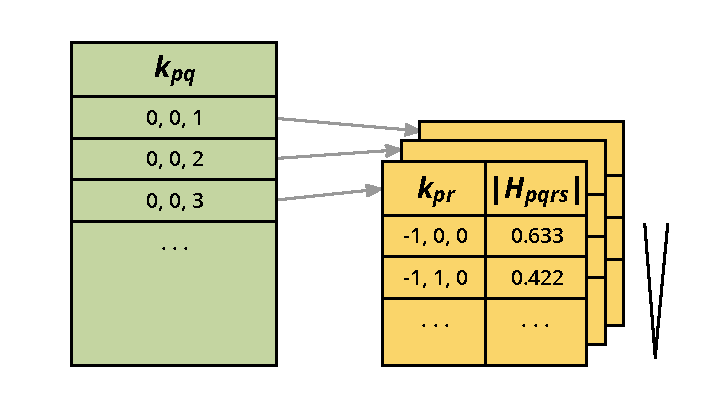
\includegraphics[width=0.9\linewidth]{figs/HelperList.eps}
  \end{center}
  \vspace{-0.2cm}
  \caption{SHCI Helper Lists for HEG.
  For each $k_{pq}$, we generate a list of $\langle k_{pr}, |H_{pqrs}|\rangle$ pairs and sort them into descending order of $|H_{pqrs}|$.
  When trying to find connected determinants from a given spawning determinant, we go through each occupied pair of orbitals $p$ and $q$, calculate their momentum difference $k_{pq}$, and go through the corresponding list until $|H_{pqrs}|$ falls below a certain threshold.
  For each entry that we go through in the list, we can obtain $r$ and $s$ by using $k_{pr}$ and momentum conservation.
  }
  \label{fig:helper}
\end{figure}

The storage complexity of these helper lists is $O(M^2)$, as opposed to $O(M^4)$ for chemistry systems.
The time complexity of finding determinants connected to a given determinant in descending order of importance is the same as in chemistry, which is $O(n_e^2 + n_D)$, where $n_e$ is the number of electrons and $n_D$ is the number of new determinants found.

\section{Results}
\label{results}
We apply our revised algorithm to HEG of several different $r_s$ values in the mid to high density region and both the 14-electron and the 54-electron supercell sizes.
In each case, we calculate the correlation energies in several basis sets of different momentum cutoffs, and perform a complete basis set (CBS) extrapolation in the end.

We notice that when the electron density is high, the correlation energies depends significantly on the momentum cutoff.
Hence, in order to obtain more accurate results, we use up to 39,886 orbitals in our calculations.
In the high density region, this decreases the CBS extrapolation distance in previous literature by about more than an order of magnitude, and thus give us much shorter extrapolation distances and more accurate results.

\subsection{14-Electron Supercell}
\begin{figure}
  \begin{center}
  \includegraphics[width=\linewidth]{figs/cbs14e_05.eps}
  \end{center}
  \vspace{-0.2cm}
  \caption{Complete basis set extrapolation for HEG 14-electron supercell with $r_s=0.5$.
  The extrapolated correlation energy is $-0.594748(12)$~Ha.
  }
  \label{fig:cbs14e_05}
\end{figure}
\begin{figure}
  \begin{center}
  \includegraphics[width=\linewidth]{figs/cbs14e_10.eps}
  \end{center}
  \vspace{-0.2cm}
  \caption{Complete basis set extrapolation for HEG 14-electron supercell with $r_s=1.0$.
  The extrapolated correlation energy is $-0.530536(18)$~Ha.
  }
  \label{fig:cbs14e_10}
\end{figure}
\begin{figure}
  \begin{center}
  \includegraphics[width=\linewidth]{figs/cbs14e_20.eps}
  \end{center}
  \vspace{-0.2cm}
  \caption{Complete basis set extrapolation for HEG 14-electron supercell with $r_s=2.0$.
  The extrapolated correlation energy is $-0.443007(12)$~Ha.
  }
  \label{fig:cbs14e_20}
\end{figure}
\begin{figure}
  \begin{center}
  \includegraphics[width=\linewidth]{figs/cbs14e_50.eps}
  \end{center}
  \vspace{-0.2cm}
  \caption{Complete basis set extrapolation for HEG 14-electron supercell with $r_s=5.0$.
  Since the correlation energy is already converged after 2000 orbitals, we use the average of the last 3 points in this case.
  The extrapolated correlation energy is $-0.30642(5)$~Ha.
  }
  \label{fig:cbs14e_50}
\end{figure}
Fig.~\ref{fig:cbs14e_05} to \ref{fig:cbs14e_50} show our CBS extrapolation curves and Table~\ref{tab:results} reports our extrapolated correlation energies.
Here $M$ is the number of spin orbitals included in a plane wave basis set.

We use quadratic extrapolations weighted by $1/M$ for $r_s$ from 0.5 to 2.0.
For $r_s=5.0$, since it is already converged at the size of the basis sets that we use, we take the average of the last three points.
\begin{table}
\caption{Summary of the HEG Total Correlation Energies~(Ha).
CCMC~\cite{neufeld2017study} uses quantum Monte Carlo to evaluate coupled cluster wavefunctions with up to 1030 orbitals and 5\nth order excitation (CCSDTQ5).
FCIQMC~\cite{shepherd2012full} and its recent improvement FCIQMC-TC~\cite{luo2018combining} use up to 2368 orbitals.
SHCI uses up to 39886 orbitals, which give shorter extrapolation distances and much more accurate results than CCMC and FCIQMC.
}
\label{tab:results}
\begin{center}
\begin{tabular}{| c || c || c | c | c | c |}
 \hline
 $r_s$ & SHCI & CCMC & FCIQMC & FCIQMC-TC \\
 \hline\hline
 0.5 & -0.594748(12) & -0.5947(2) & -0.5959(7) & -0.5948(2)\\
 \hline
 1.0 & -0.530536(18) & -0.5311(2) & -0.5316(4) & -0.5309(2)\\
 \hline
 2.0 & -0.443007(12) & -0.4434(10) & -0.444(1) & -0.4440(3)\\
 \hline
 5.0 & -0.30642(5) & -0.3025(4) & -0.307(1) & -0.3078(3)\\
 % DMC~\cite{rios2006inhomogeneous}
%  \hline
%  54 & 0.5 & -2.4316(6) & - & -2.435(7) & -2.387(2) \\
%  \hline
%  54 & 1.0 & -2.114(2) & - & -2.124(3) &  -2.125(2) \\
 \hline
\end{tabular}
\end{center}
\end{table}

We can see from this table that the results from SHCI are significantly more accurate than previous results.
This is mainly due to the fact that the high performance of SHCI and its capability to work with large basis sets enable us to go much closer to the infinite basis set. Fig.~\ref{fig:comparison} which plots the raw data points from FCIQMC~\cite{shepherd2012full} and SHCI, illustrates this.
\begin{figure}
  \begin{center}
  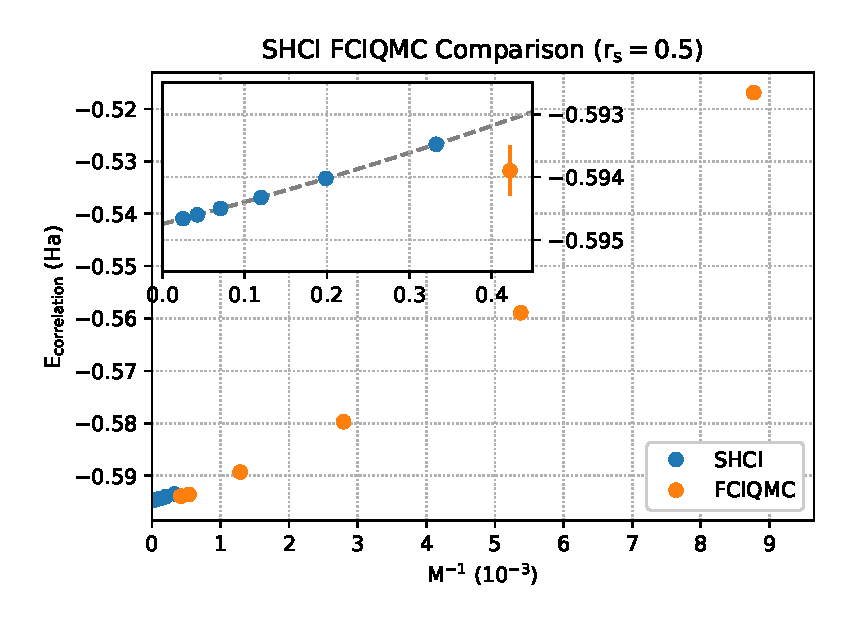
\includegraphics[width=\linewidth]{figs/compare.eps}
  \end{center}
  \vspace{-0.2cm}
  \caption{Comparison between SHCI results and FCIQMC results for $r_s=0.5$.
  Note that all the points have error bars smaller than the size of the points themselves except for the FCIQMC point on the zoomed-in view.
  SHCI goes much closer to the infinite basis set and thus achieves more accurate and reliable extrapolated results.
  }
  \label{fig:comparison}
\end{figure}

\subsection{54-Electron Supercell}
We also apply SHCI to the 54-electron supercell case.
Fig.~\ref{fig:cbs54e_05} shows the CBS extrapolation and Table~\ref{tab:results54} compares the SHCI results with FCIQMC and DMC.

We can see that our SHCI result agrees well with FCIQMC, but slighly lower than FCIQMC-TC, and all of them are much higher then BF-DMC, which probably used a poor trail wavefunction.
In these SHCI calculations, we use an order of magnitude more orbitals than FCIQMC and FCIQMC-TC, and the extrapolation distance of SHCI is about an order of magnitude smaller than FCIQMC and 4 times smaller than FCIQMC-TC.
Hence, we believe the extrapolated value from SHCI is likely to be more accurate and reliable than both FCIQMC and FCIQMC-TC.

\begin{figure}
  \begin{center}
  \includegraphics[width=\linewidth]{figs/cbs54e_05.eps}
  \end{center}
  \vspace{-0.2cm}
  \caption{Complete basis set extrapolation for HEG 54-electron supercell with $r_s=0.5$.
  The extrapolated correlation energy is $-2.4313(11)$~Ha.
  }
  \label{fig:cbs54e_05}
\end{figure}
\begin{table}
\caption{Summary of the HEG Total Correlation Energies~(Ha) with 54-Electron Supercells.
DMC~\cite{rios2006inhomogeneous} uses real space basis and backflow wave function.
FCIQMC~\cite{shepherd2012full} and its recent improvement FCIQMC-TC~\cite{luo2018combining} use up to 1850 orbitals.
SHCI uses up to 23506 orbitals, which give much shorter extrapolation distances than FCIQMC and thus more accurate results.
}
\label{tab:results54}
\begin{center}
\begin{tabular}{| c || c || c | c | c | c |}
 \hline
 $r_s$ & SHCI & FCIQMC & FCIQMC-TC & BF-DMC \\
 \hline\hline
 0.5 & -2.4313(11) & -2.435(7) & -2.425(1) & -2.387(2) \\
 \hline
 % DMC~\cite{rios2006inhomogeneous}
%  \hline
%  54 & 0.5 & -2.4316(6) & - & -2.435(7) & -2.387(2) \\
%  \hline
%  54 & 1.0 & -2.114(2) & - & -2.124(3) &  -2.125(2) \\
 \hline
\end{tabular}
\end{center}
\end{table}

\section{Conclusion}
In this paper, we apply our fast semistochastic heat-bath configuration interaction algorithm (SHCI) to the homongenous electron gas (HEG) problem in the mid to high density region.
The basis set incompleteness error is a dominating error in this region, and the uncertainty of the result depends a lot on the uncertainty of the extrapolation, which in terms depends on the extrapolation distance.
By using SHCI with up to 39886 orbitals, we reduce the extrapolation distance significantly and achieves more accurate results than state-of-the-art methods.

\label{conclusions}


\chapter{Chromium Dimer Simulation with Fast SHCI}
In this chapter, I apply the fast SHCI method to the chromium dimer system.
I first perform an accurate calculation at the equilibrium geometry, and then perform a slightly less accurate calculation for several squeezed or stretched geometries and obtain the entire potential energy surface.

\section{Introduction}

Chromium dimer is a challenging strongly-correlated system
that has been used as a benchmark molecule for a variety of methods~\cite{Scu-JCP-91,KurYan-JCP-11,PurZhaKra-JCP-15,MaManOlsGag-JCTC-16,VanMalVer-JCTC-16,GuoWatHuSunCha-JCTC-16}.
In this chapter, we use the fast heat-bath configuration interaction method to calculate both the energy at the equilibrium geometry and entire potential energy curve.

For the equilibrium geometry, we include in our variational wavefunction two billion most important determinants, which are two orders of magnitudes more than ever done in other selected-CI based methods.
This allows us to achieve significantly higher accuracy, which even beats the accuracy of well-developed methods, such as the density matrix renormalization group (DMRG).
Section~\ref{sec:eq} presents the results.

%For the entire potential energy curve calculation, we include in our Hilbert space up to 28 active electrons with a cc-pVDZ basis.
For the entire potential energy curve calculation, we correlate up to 28 electrons in a cc-pVDZ basis.
The resulting Hilbert space of $5 \times 10^{29}$ determinants is several orders of magnitude larger than that used in other
systematically improvable methods.
Our results match well with the experiments at and near the equilibrium geometry.
Section~\ref{sec:curve} presents the results.

\section{Equilibrium Geometry}
\label{sec:eq}
In this section, we examine the chromium dimer at the equilibrium bond length of 1.68 $\AA$. % angstroms.
%We use a cc-pVDZ basis with active semi-core electrons.
We use a relativistic exact two-component (X2C) Hamiltonian, the cc-pVDZ-DK basis, and we correlate the valence and the semi-core electrons.
This gives an active space of (28e, 76o) and a Hilbert space of $5\times10^{29}$ determinants, which is far beyond the reach of FCI.
We show how we obtain an accurate estimate of the FCI energy in this large active space with our improved SHCI algorithm.

We use PySCF~\cite{SunCha_etal_PySCF-ComMolSci-18} to generate the molecular orbital integrals for orbitals that minimize the HCI variational
energy for $\epsilon_1=2\times 10^{-4}$~Ha, using the method of Ref.~\cite{SmiMusHolSha-JCTC-17}.
We perform SHCI with several $\epsilon_1$ values from $5\times10^{-5}$ to $3\times10^{-6}$~Ha.
The Hamiltonian matrix is constructed only once.
% The Hamiltonian matrix is stored in memory and so needs to be constructed only once.
%We keep the ratio between $\epsilon_2$ and $\epsilon_1$ to $10^{-6}$ and the target error for the stochastic perturbation to 0.01 mHa.
We use very small values of $\epsilon_2 = 10^{-6} \epsilon_1$  to ensure that the perturbative correction is exceedingly well converged,
and choose the target error for the stochastic perturbation energy to be $10^{-5}$~Ha.

%The improved SHCI is fast enough that we can use over two billion variational determinants and include at least trillions of effective perturbative determinants.
The improved SHCI is fast enough that we can use over two billion variational determinants, and stochastically include the contributions of at least trillions of perturbative determinants.
The largest variational calculation, where we iteratively find and diagonalize 2 billion determinants
for $\epsilon_1=3.0\times10^{-6}$~Ha, takes only one day on 8 nodes, each of which has 4 Intel Xeon E7-8870 v4 CPUs.
The corresponding perturbative calculation takes only 6 hours using only one of these nodes. 
During that perturbative calculation, we skip the deterministic step, perform a pseudo-stochastic step with $\epsilon_2^{\rm psto}=1\times10^{-7}$~Ha, and a stochastic step with $\epsilon_2=3\times10^{-12}$~Ha.
{\color{black}
We skip the deterministic step here because $\epsilon_1=3 \times 10^{-6}$ is already close to our
default $\epsilon_2^{\rm dtm}$ of $2 \times 10^{-6}$ so skipping this won't affect the efficiency
of subsequent steps much.
}
The pseudo-stochastic step uses 25 batches, each of which has about 8.9 billion determinants.
We evaluate only one of them, from which we obtain an estimate of the total correction for all the 25 batches (223 billion determinants) to be -0.011681(1)~Ha.
Since the estimated error is already much smaller than our target error, we skip the remaining 24 batches.
The pseudo-stochastic step takes 1.6 hours.
The stochastic step uses 128 batches and 6 million variational determinants in each sample,
which results in about 3.7 billion determinants per batch.
We use 10 samples and obtain the additional correction from $\epsilon_2=3.0\times10^{-12}$~Ha to be -0.001203(6)~Ha.
The combined uncertainty of the entire semistochastic perturbation stage is 6~$\mu$Ha.
It is hard to estimate how many determinants are stochastically included for $\epsilon_2=3\times10^{-12}$~Ha,
so we estimate a lower bound with $\epsilon_2^{\rm psto}=1.4\times10^{-8}$~Ha and obtain 1.8 trillion unique perturbative determinants.
Hence, with $\epsilon_2=3\times10^{-12}$~Ha (the value we are actually using) we stochastically estimate contributions from
at least trillions of unique perturbative determinants and obtain better than $10^{-5}$~Ha statistical uncertainty in 6 hours using only one node.
%why?
%This brings the accuracy selected-CI to a whole new level and enables us to obtain an estimation of the FCI energy with sub-millihartree uncertainty in this large active space.

These large calculations enable us to obtain an estimate of the FCI energy with sub-millihartree uncertainty in this large active space.
Table~\ref{tab:Cr2} reports the results.


\begin{table}
  \begin{center}
  \begin{tabular}{| c | c | c | c |}
  \hline
  $\epsilon_{1}$ (Ha) & $N_\V$ & $E_{\rm var}$ (Ha) & $E_{\rm total}$ (Ha) \\
  \hline\hline
  $5.0\times10^{-5}$ & 24M & -2099.863816 & -2099.909741(7) \\
  \hline
  $3.0\times10^{-5}$ & 53M & -2099.875327 & -2099.912356(7) \\
  \hline
  $2.0\times10^{-5}$ & 102M & -2099.883027 & -2099.914132(8) \\
  \hline
  $1.0\times10^{-5}$ & 309M & -2099.893761 & -2099.916595(1) \\
  \hline
  $7.0\times10^{-6}$ & 539M & -2099.898165 & -2099.917540(1) \\
  \hline
  $5.0\times10^{-6}$ & 911M & -2099.901781 & -2099.918306(3) \\
  \hline
  $3.0\times10^{-6}$ & 2.00B & -2099.906322 & -2099.919205(6) \\
  \hline
  0.0 (Extrap.) & - & \multicolumn{2}{ c |}{-2099.9224(6)} \\
  \hline
  \end{tabular}
  \end{center}
  \caption{Results for Cr$_2$ at r=1.68\AA\ in the cc-pVDZ-DK basis.
  The active space is (28e, 76o).
  $N_\V$ is the number of variational determinants.
  $\epsilon_2 = 10^{-6} \epsilon_1$.
  We use weighted quadratic extrapolation, shown in Fig.~\ref{fig:extrapolation}, to obtain the FCI limit
  corresponding to $\Delta E=0$.}
  \label{tab:Cr2}
\end{table}

\begin{figure}
  \includegraphics[width=\linewidth]{figs/extrapolate.eps}
  \caption{Weighted quadratic extrapolation of the Cr$_2$ ground state energy.
  The weight of each point is $(E_{\rm var} - E_{\rm tot})^{-2}$.
  The extrapolated energy is $-2099.9224(6)$, where the uncertainty comes from the difference between linear extrapolation and quadratic extrapolation.
  The p-DMRG extrapolation and the CCSD(T) value are also shown.
  {\color{red} I don't remember -- where did this CCSD(T) value come from?  Does it matter if it is CCSD(T) or UCCSD(T)?}
}
  \label{fig:extrapolation}
\end{figure}

We extrapolate our results using a weighted quadratic fit
and obtain for the ground state energy, $-2099.9224$~Ha as $\Delta E\to0$.
The weight of each point is $(E_{\rm var} - E_{\rm tot})^{-2}$.
Fig.~\ref{fig:extrapolation} shows the computed energies and the extrapolation.
We also perform a weighted linear fit and use the difference of the extrapolated values from the quadratic and the linear fits (0.6~mHa) as the uncertainty.
%If we look at the trends of the data points in Fig.~\ref{fig:extrapolation}, we can see that 0.55~mHa is a reasonable estimation of the uncertainty.
%In summary, the estimated FCI energy of Cr$_2$ in the cc-pVDZ basis with active semi-core electrons is $-2099.9224(6)$~Ha.
In summary, the estimated FCI energy of Cr$_2$ in the cc-pVDZ-DK basis with 28 correlated electrons and the relativistic X2C Hamiltonian
%(the rest of the electrons are frozen in
%Hartree-Fock orbitals)
is $-2099.9224(6)$~Ha.

\begin{figure}
  \begin{center}
  \includegraphics[width=0.9\linewidth]{figs/excitation.eps}
  \caption{Contribution from each excitation level to the variational wavefunction for Cr$_2$ with $2 \times 10^9$ determinants.
  Determinants with up to 15 excitations are present in the variational wavefunction.
%  {\color{red} Leave out the top plot, since sums of squared magnitudes is meaningful, but number of nonzero magnitudes is a meaningless quantity? Well, it does mean that there were several higher-order excitations that are more important than lower-order ones.}
}
  \label{fig:excit}
  \end{center}
\end{figure}

We compare our result with DMRG and p-DMRG, which are the only essentially exact methods that have been applied to this large active space of the chromium dimer.
The DMRG calculations use up to bond dimension $M=16000$ and obtain an extrapolated energy of $-2099.9195(27)$~Ha (default schedule) and $-2099.9192(24)$ (reverse schedule)~\cite{GuoLiCha-JCTC-18}.
%These two values are similar to our most accurate data point but higher than our extrapolated result by 3~mH, which is about one standard error of the DMRG results.
These two values are similar to our most accurate data point but higher than our extrapolated result by 3~mH, which is about the estimated error of the DMRG results.
%The p-DMRG calculations use up to $M=4000$ and obtain an extrapolated energy of $-2099.9201$~Ha~\cite{GuoLiCha-JCTC-18}.
The p-DMRG calculations use up to $M=4000$ and extrapolated energy obtained from a linear fit is $-2099.9201$~Ha~\cite{GuoLiCha-JCTC-18}.
If instead, we perform a weighted quadratic fit (shown in Fig.~\ref{fig:extrapolation}), the extrapolated energy is $-2099.9225$~Ha,
in perhaps fortuitously good agreement with our result of $-2099.9224(6)$~Ha.  However, the extrapolation uncertainty is larger than the SHCI extrapolation uncertainty.
In contrast, the CCSD(T) energy is considerably higher.
%In summary, our extrapolated value agrees with DMRG's and p-DMRG's extrapolated results but we achieve a smaller uncertainty.

%One of the merits of selected-CI is the ability to take higher-order excitations into account accurately.
%One of the merits of selected-CI methods is the ability to include higher-order excitations.
One of the merits of selected-CI methods is the ability to include all excitations, regardless of excitation level.
To see the contribution from each excitation level we plot the number of selected determinants and the $\sum_i \left|c_i\right|^2$ versus excitation level in Fig.~\ref{fig:excit}.
Determinants with excitation levels up to 15 excitations are present in the variational wavefunction even though we are using optimized orbitals.
(Using Hartree-Fock orbitals, we expect that determinants with even higher excitation levels will be present.)
%This implies that truncating the CI or the CC at the double or the triple excitation level may not give reliable results for such strongly correlated systems.
This implies that truncating the CI expansion at the double, triple or quadruple excitation levels (which is the most that is usually done in systematic
CI expansions), will give poor energies for such strongly correlated systems.

\section{Potential Energy Surface}
In addition to the energy at equilibrium geometry, I also obtain the entire potential energy curve of the chromium dimer.

We calculate the potential energy curves, first correlating just the 12 valence (3d, 4s) electrons, and then correlating
also the semi-core (3s,
3p) electrons, making a total of 28 correlated electrons.
For 12 correlated electrons, we study the basis set dependence by calculating the curves for cc-pVDZ, cc-pVTZ and cc-pVQZ basis sets.
%We examine the effect of correlating the semi-core electrons, i.e., we
%We exam the results from using the cc-pVDZ-DK basis and the cc-pVTZ-DK basis, and also the effects of correlating only the 12 valence electrons and correlating 28 electrons from both the valence and the semi-core.
The largest active space in our calculations is (28e, 76o), which gives a Hilbert space of $5\times10^{29}$ determinants, far beyond the reach of FCI.
%Due to the high efficiency of our algorithm, we can calculate each data point on this curve with such huge active space and obtain the entire potential energy curve.

We use both PySCF~\cite{SunCha_etal_PySCF-ComMolSci-18} and our program to generate the molecular orbital integrals for orbitals that minimize the HCI variational
energy for $\epsilon_1=2\times 10^{-4}$~Ha, using an improved version of the method of Ref.~\cite{SmiMusHolSha-JCTC-17}.
For 12 correlated electrons, we use the CAS core optimized orbitals, and for 28 correlated electrons, we use the HF core.
We perform SHCI with several $\epsilon_1$ values from $2\times10^{-4}$ to $5\times10^{-6}$~Ha.
%The Hamiltonian matrix is constructed only once for each geometry and each active space.
The sparse Hamiltonian matrix is stored in memory and so needs to be constructed only once for each geometry and each active space.
%We keep the ratio between $\epsilon_2$ and $\epsilon_1$ to $10^{-6}$ and the target error for the stochastic perturbation to 0.01 mHa.
For the perturbative correction calculation, we set $\epsilon_2 = 0$  to include the entire Hilbert space.

%The improved SHCI is fast enough that we can use over two billion variational determinants and include at least trillions of effective perturbative determinants.
The improved SHCI is fast enough that we can use more than one billion variational determinants and stochastically include the corrections from at least trillions of perturbative determinants for each geometry.

We extrapolate the energies for each geometry with a weighted quadratic fit
and obtain for the ground state energy as $\Delta E\to0$.
The weight of each point is $(E_{\rm var} - E_{\rm tot})^{-2}$.
Then we interpolate the points for each active space with cubic spline interpolation.

\label{sec:curve}
\begin{figure}
  \begin{center}
  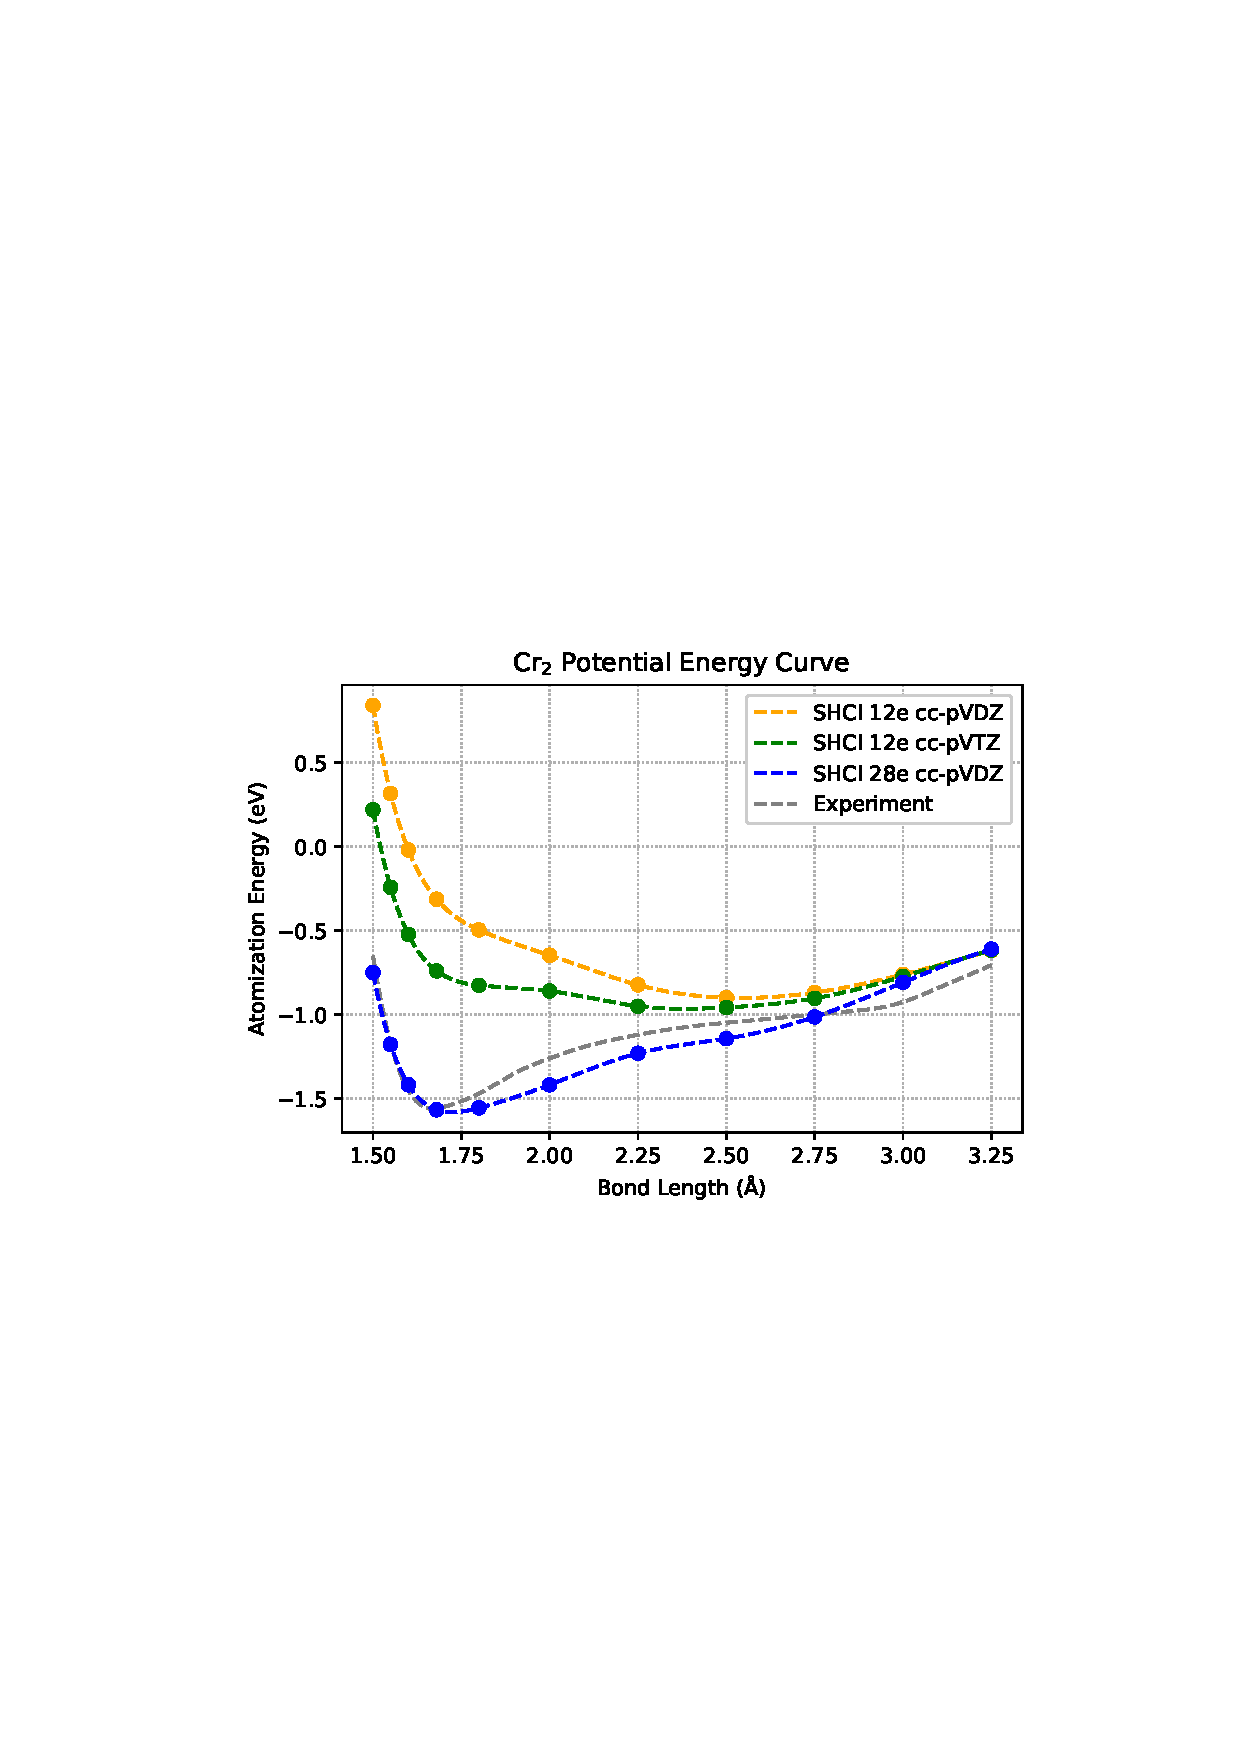
\includegraphics[width=0.9\linewidth]{figs/cr2curve.png}
  \caption{Comparison of SHCI potential energy curves of Cr$_2$, correlating 12 or 28 electrons, with experiment.
  The shape of the experimental data is deduced from measuring 29 vibrational states using negative-ion photoelectron spectroscopy~\cite{casey1993negative}.
  %We can see that using only 12 active electrons from the shell cannot produce a good agreement to the experimental data.
  %By including 10 additional electrons from the semi-core into the active space, the agreement with experimental data is much better.
  The potential energy curves from the 12-correlated-electron calculations agree poorly with experiment, though the agreement
  improves upon increasing the basis size.
  The 28-correlated-electron calculation agrees much better with experiment.
   {\color{red} For the 12-electron curves you should keep in the Fig. legend CAS-core, since for 12 electrons
there is a large difference between CAS and HF cores.}
  }
  \label{fig:cr2curve}
  \end{center}
\end{figure}

\begin{figure}
  \begin{center}
  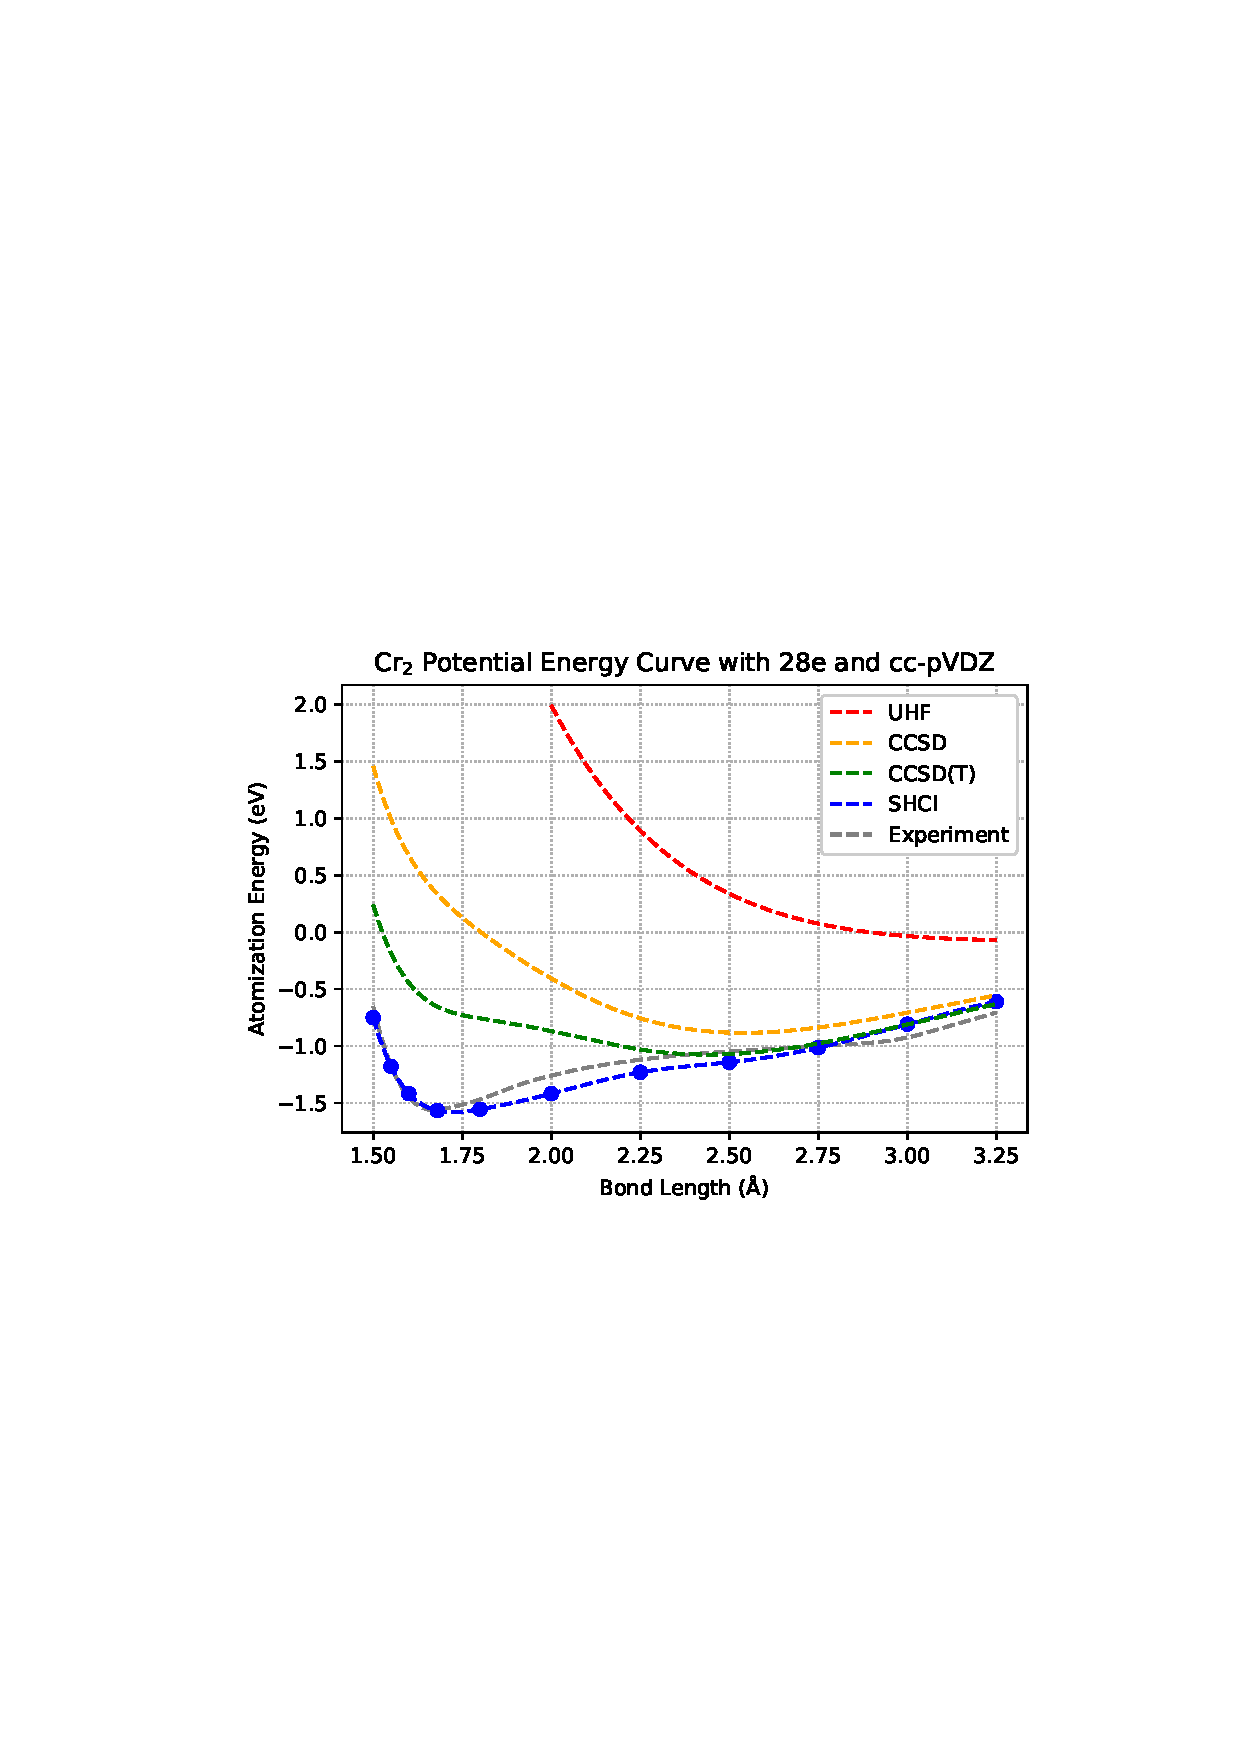
\includegraphics[width=0.9\linewidth]{figs/hfcc.png}
  \caption{Potential energy curve of Cr$_2$ with 28 electrons in a cc-pVDZ basis calculated from various methods.
  The experimental data come from negative-ion photoelectron spectroscopy~\cite{casey1993negative}.
  %We can see that using UHF and CCSD cannot produce a good agreement to the experimental data.
  %CCSD(T) can produce better agreement at stretched geometry but still not good enough near the equilibrium geometry.
  %By using SHCI, the agreement with experimental data is much better.
  The UHF curve bears no resemblance to the experimental curve.
  The UCCSD and UCCSD(T) curves are better, especially at long bond lengths, but even UCCSD(T) which is considered to be the ``gold standard" for single-reference
  systems, agrees poorly with experiment.  In contrast the SHCI curve is in reasonable agreement with experiment.
}
  \label{fig:hfcc}
  \end{center}
\end{figure}

Fig.~\ref{fig:cr2curve} compares the energies calculated with different active spaces to the experimental data.
There is some uncertainty in the experimental curve due to uncertainty in the assignment of the higher vibrational levels
as well as due to uncertainty in the depth of the potential.
The shape of the experimental curve is deduced from 29 vibrational states using negative-ion photoelectron spectroscopy~\cite{casey1993negative}.
The measured 29 vibrational states were assigned to $\nu=1-9$ and $\nu=24-43$.
There is uncertainty in the shape of the experimental curve because of the missing vibrational levels as well as uncertainty
about the assignment of the observed peaks to the higher vibrational levels.
The depth of the experimental curve is estimated from adding an estimate of the zero-point energy
to experimentally determined bond dissociation energies.
Unfortunately there is a considerable spread in the estimates of the latter.
Here we use the well depth estimate of 1.56 eV from Ref.~\cite{VanMalVer-JCTC-16}, which is based on the bond dissociation
energy of Ref.~\cite{simard1998photoionization}.
This well depth is deeper than the estimate of 1.47 eV used in Ref.~\cite{GuoWatHuSunCha-JCTC-16} based on
the bond energy of 1.44 eV reported in Ref.~\cite{casey1993negative}.

Fig..~\ref{fig:cr2curve} shows that the 12-active-electron curves do not agree well with experiment.
Using a larger basis sets helps bring the curve closer to the experimental data, but is not enough to produce a good agreement.
By including the 10 additional electrons from the semi-core in the active space, SHCI achieves much better agreement,
demonstrating that semi-core correlation plays an important role in the molecular bond of Cr$_2$.
At large bond lengths one would expect that semi-core correlation is not important and in fact the 12 active electron
and the 28 active electron energies become nearly coincident there.

% We can also see from Fig.~\ref{fig:cr2curve} that the effect of using HF core or CAS core for orbital optimization matters little to the 28 electrons SHCI calculation.

%We also compare SHCI results with unrestricted Hartree-Fock (UHF) and low order coupled cluster methods.
In Fig.~\ref{fig:hfcc}, we compare SHCI results to unrestricted Hartree-Fock (UHF) and unrestricted coupled cluster methods, UCCSD and UCCSD(T).
%Fig.~\ref{fig:hfcc} shows the comparison.
%We can see UHF cannot give a good agreement with the experimental data.
%CCSD and CCSD(T) give better agreements for the stretched geometries, but still cannot reach good agreements with the experimental data at compressed or equilibrium geometries.
%SHCI gives good agreement to the experimental data along the entire curve.
As expected, the UHF curve bears no resemblance to the experimental curve.
The UCCSD and UCCSD(T) curves are better, but even UCCSD(T) which is considered to be the ``gold standard" for single-reference
systems, agrees poorly with experiment.  In contrast the SHCI curve is in reasonable agreement with experiment, perhaps
fortuitously so, since the cc-pVDZ basis used is expected to have a significant finite-basis error.
With our current computer resources, we cannot obtain a well converged curve with larger basis sets,
but with further improvements in the method and larger computers we hope to obtain basis set converged curves
that agree yet better with experiment, and perhaps even provide information about experimental inaccuracies.

%Given the resources that we have right now, 28 electrons in a cc-pVDZ basis are the largest configuration that we can do for the entire potential energy curve.
%In the future, as our method keep evolving, and we get more computing resources, we expect SHCI to give even better agreement to the experimental data and can even be used to benchmark the accuracy of experiments on stretches geometries.

\chapter{Simplified High Performance Cluster Computing}
MapReduce and its variants have significantly simplified and accelerated the process of developing parallel programs.
However, most MapReduce implementations focus on data-intensive tasks while many real-world tasks are compute intensive and their data can fit distributedly into the memory.
For these tasks, the speed of MapReduce programs can be much slower than those hand-optimized ones.
We present Blaze, a C++ library that makes it easy to develop high performance parallel programs for such compute intensive tasks.
At the core of Blaze is a highly-optimized in-memory MapReduce function, which has three main improvements over conventional MapReduce implementations:
eager reduction, fast serialization, and special treatment for a small fixed key range.
We also offer additional conveniences that make developing parallel programs similar to developing serial programs.
These improvements make Blaze an easy-to-use cluster computing library that approaches the speed of hand-optimized parallel code.
We apply Blaze to some common data mining tasks, including word frequency count, PageRank, k-means, expectation maximization (Gaussian mixture model), and k-nearest neighbors.
Blaze outperforms Apache Spark by more than 10 times on average for these tasks, and the speed of Blaze scales almost linearly with the number of nodes.
In addition, Blaze uses only the MapReduce function and 3 utility functions in its implementation while Spark uses almost 30 different parallel primitives in its official implementation.

\section{Introduction}

Cluster computing enables us to perform a huge amount of computations on big data and get insights from them at a scale that a single machine can hardly achieve.
However, developing parallel programs to take advantage of a large cluster can be very difficult.

\begin{figure}
  \begin{center}
  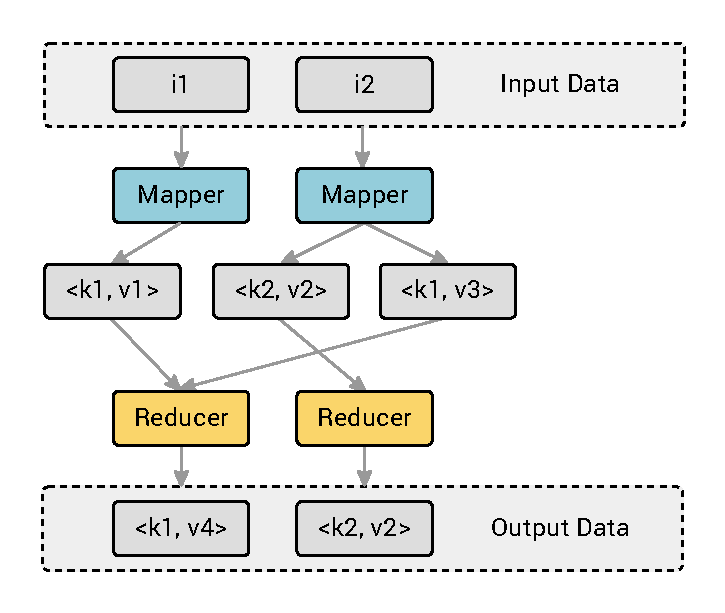
\includegraphics[width=0.7\linewidth]{figs/mr0.eps}
  \end{center}
  \vspace{-0.2cm}
  \caption{MapReduce Programming Model.
  The map function generates a set of intermediate key/value pairs for each input.
  The reduce function merges the values associated with the same key.
  Numerous data mining and machine learning algorithms are expressible with this model.
  }
  \label{fig:mr}
\end{figure}

MapReduce~\cite{dean2008mapreduce,dean2010mapreduce} greatly simplified this task by providing users a high-level abstraction for defining their computation, and taking care of the intricate low-level execution steps internally.
Fig.~\ref{fig:mr} illustrates the MapReduce programming model.
Logically, each MapReduce operation consists of two phases: a map phase where each input is mapped to a set of intermediate key/value pairs, and a reduce phase where the pairs with the same key are put together and reduced to a single key/value pair according to a user specified reduce function.


Many data mining algorithms are expressible with this model, such as PageRank~\cite{bahmani2011fast,plimpton2011mapreduce,ekanayake2010twister}, k-means~\cite{zhao2009parallel,chu2007map,cui2014optimized,anchalia2013mapreduce,gopalani2015comparing}, Gaussian mixture model~\cite{chu2007map}, and k-nearest neighbors~\cite{anchalia2014k,maillo2015mapreduce,lu2012efficient,yokoyama2012processing}.

Although logically expressible, achieving similar efficiency as a hand-optimized parallel code is hard, especially when the data can be fit distributed into the memory.
In such cases, the file system is no longer the bottleneck and the overhead from MapReduce can make the execution much slower than hand-optimized code.

Google's MapReduce~\cite{dean2008mapreduce,dean2010mapreduce} and most of its variants~\cite{hadoop,chambers2010flumejava,cascading,afrati2010optimizing,bhatotia2011incoop,condie2010mapreduce,ekanayake2010twister,goiri2015approxhadoop,he2008mars,li2015coded,zaharia2008improving,yang2007map} save intermediate data and result to the file system even when the data can be fit into the memory.
Hence, its MapReduce performance is severely limited by the performance of the file system.

Spark~\cite{spark, zaharia2010spark, zaharia2016apache, zaharia2012resilient} offers an in-memory implementation of MapReduce, which is much faster than Google's MapReduce.
However, it uses a similar algorithm as Google's MapReduce, which is designed for disk-based data intensive use cases and does not consider the computational overheads of MapReduce seriously.
Hence, the performance of Spark is often far from the performance of hand-optimized code.

To achieve better performance while preserving the high-level MapReduce abstraction, we develop Blaze, a C++ based cluster computing library that focuses on in-memory high performance MapReduce and related operations.
Blaze introduces three main improvements to the MapReduce algorithm: eager reduction, fast serialization, and special treatment for a small fixed key range.
Section~\ref{sec:opt} provides a detailed description of these improvements.

We apply Blaze to several common data mining tasks, including word frequency count, PageRank, k-means, expectation maximization (Gaussian mixture), and k-nearest neighbors.
Our results show that Blaze is on average 10 times faster than Spark on these tasks.
% We compare its performance with Apache Spark and results

The main contributions of this research are listed as follows:
\begin{enumerate}
    \item We develop Blaze, a high performance cluster computing library that allows users to write parallel programs with the high-level MapReduce abstraction while achieving similar performance as hand-optimized code for compute intensive tasks.
    \item We introduce three main performance improvements to the MapReduce algorithm to make it more efficient: eager reduction, fast serialization, and special treatment for a small fixed key range.
    \item We apply Blaze to 5 common data mining tasks and demonstrate that Blaze programs are easy to develop and can outperform Apache Spark programs by more than 10 times on average for these tasks.
    % by applying the improvements above, we can keep the simple high-level abstraction of MapReduce while achieving $10 \times$ higher performance than Apache Spark on some common data mining and machine learning tasks.
\end{enumerate}

The remaining sections are organized as follows:
Section~\ref{sec:blaze} describes the Blaze framework and the details of the optimization.
Section~\ref{sec:app} present the details of how we implement several key data mining and machine learning algorithms with Blaze and compare the performance with Apache Spark.
Section~\ref{sec:con} concludes the paper.

\section{The Blaze Library}
\label{sec:blaze}
The Blaze library offers three sets of APIs: 1) a high-performance MapReduce function, 2) distributed data containers, and 3) parallel computing utility functions.
These APIs are built based on the Blaze parallel computing kernel, which provides common low-level parallel computing primitives.

% Blaze also offers several utility functions for parallel programming, including thread-safe random number generators, a parallel file loader, and converters between C++ standard library containers and Blaze distributed data containers.


\begin{figure}
  \begin{center}
  \includegraphics[width=0.7\linewidth]{figs/arch0.eps}
  \end{center}
  \vspace{-0.2cm}
  \caption{Blaze Architecture.
%   Blaze exposes three sets of APIs: the high performance Blaze MapReduce function, distributed data containers, and a few utility functions.
%   The Blaze parallel computing kernel provides low-level parallel computing primitives to support the high-level APIs.
  }
  \label{fig:mrdiff}
\end{figure}

\subsection{Distributed Containers}

Blaze provides three distributed data containers: \emph{DistRange}, \emph{DistVector}, and \emph{DistHashMap}.
DistRange does not store the whole data but only the start, the end, and the step size of the data.
DistVector distributedly stores an array of elements.
DistHashMap distributedly stores key/value pairs.

All of the three containers support the \lstinline{foreach} operation, where a custom function can be applied to each of its element in parallel.
This function can either change the value of the element itself or use the value of the element to perform external operations.

Both the DistVector and the DistHashMap can be converted to and from C++ standard library containers with Blaze utility functions \lstinline{distribute} and \lstinline{collect}.
DistVector can also be created from the \lstinline{load_file} utility function, which can load text files from the file system parallelly into a distributed vector of lines.

DistVector also has a \lstinline{topk} method, which can return the top k elements from the distributedly stored vector in $O(n+k\log k)$ time and $O(k)$ space.
Users can provide a custom comparison function to determine the priority of the elements.

\subsection{MapReduce}

The MapReduce function uses a functional style interface.
It takes four parameters:
\begin{enumerate}
    \item Input. One of the Blaze distributed container.
    \item Mapper. When the input is a DistRange, the mapper should be a function that accepts two parameters: a value from the DistRange and a handler function for emitting key/value pairs.
    When the input is a DistVector or a DistHashMap, the mapper should be a function that accepts three parameters: a key from the input, the corresponding value, and an emit handler.
    \item Reducer. The function that reduce two values to one value.
    Blaze provides several built-in reducers, including \lstinline{sum}, \lstinline{prod}, \lstinline{min}, and \lstinline{max}, which can cover most use cases.
    These reducers can be used by providing the reducer name as a string, for example, \lstinline{"sum"}.
    Users can also provide custom reduce functions, which should take two parameters, the first one is a reference to the existing value which needs to be updated, and the second one is a constant reference to the new value.
    \item Target. One of the Blaze distributed container or a vector from the standard library.
    The target container should be mutable and it is not cleared before performing MapReduce.
    New results from the MapReduce operation are merged/reduced into the target container.
\end{enumerate}

Blaze MapReduce also takes care of the serialization of common data types so that the map function can emit non-string key/value pairs, and the reduce function no longer requires additional logic for parsing the serialized data.
Using custom data types as keys or values is also supported. For that, users only need to provide the corresponding serialize/parse methods and a hash function (for keys).

We provide two examples of using Blaze MapReduce in section ~\ref{app:wordcount} and \ref{app:pi}.

\subsection{Optimization}
\label{sec:opt}
We introduce several optimizations to make the MapReduce function faster, including eager reduction, fast serialization, and special treatment for cases where the resulting key range is small and fixed.

\subsubsection{Eager Reduction}

Conventional MapReduce performs the map phase first and saves all the emitted pair from the mapper function.
Then, it shuffles all the emitted pairs across the networks directly, which could incur a large amount of network traffics.

\begin{figure}
  \begin{center}
  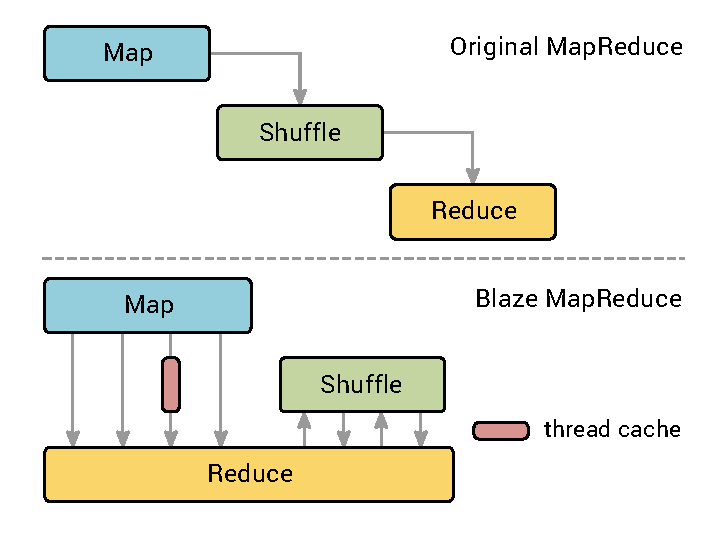
\includegraphics[width=0.7\linewidth]{figs/mrDiff0.eps}
  \end{center}
  \vspace{-0.2cm}
  \caption{Eager Reduction in Blaze MapReduce.
%   Blaze performs machine-local reduce right after the mapper function emits a key/value pair.
%   For popular keys, Blaze automatically reduce new values to a thread-local cache instead of the main copy on a machine.
%   The cross-machine shuffle operates on the locally reduced data and thus requires much less network communication.
%   During the shuffle operations, reduce operations also happen asynchronously to maximize the throughput.
  }
  \label{fig:mrdiff}
\end{figure}

In Blaze MapReduce, we perform machine-local reduce right after the mapper function emits a key/value pair.
For popular keys, Blaze automatically reduces new values to a thread-local cache instead of the machine-local copy.
The cross-machine shuffle operates on the locally reduced data which substantially reduces the network communication burden.
During the shuffle operations, reduce functions are also operating asynchronously to maximize the throughput.
Fig.~\ref{fig:mrdiff} illustrates the difference between the conventional MapReduce and Blaze MapReduce with eager reduction.

\subsubsection{Fast Serialization}
During the shuffle/reduce phase, we serialize the messages into a compact binary format before casting them across the network.

Although these two fields allow missing fields and support serializing the fields in arbitrary order, this additional flexibility is not needed in MapReduce.
On the other hand, these two fields can have a significant impact on both the performance and the serialized message size, especially when the content size of a field is small, which is common for MapReduce key/value pairs.
For example, when both the key and value are small integers, the serialized message size of each pair from Protocol Buffers will be 4 bytes while the message from Blaze fast serialization will be only 2 bytes, which is 50\% smaller than the one from Protocol Buffers.
Removing the fields tags and wire types does not cause ambiguity as long as we always serialize the fields in the same order, which is easy to achieve in MapReduce.
The smaller size in the serialized message means less network traffics, so that Blaze can scale better on large clusters when the cross-rack bandwidth becomes the bottleneck.

% \subsubsection{Hash-Based Shuffle}

% We use hash based shuffle instead of the original sort based shuffle.
% Hash based shuffle can send the messages to the corresponding worker in $O(1)$ time.

% Note that in the MapReduce results, the keys are no longer sorted.
% We provide a separate function, called \lstinline{top} for achieving similar capability in the distributed vector container.
% \lstinline{top} returns the top k elements in the distributed vector container in $O(n + k \log k)$ time, according to a custom compare function.
% When $k=n$, it will essentially perform a parallel merge sort.
% In section \ref{sec:nn}, we provide an example of the nearest 100 neighbors related to a given point from a huge set of other points, which uses the member function.

\subsubsection{Optimization for Small Key Range}

For small key range, we create a thread-local cache for each key at the beginning and set that as the reduce target during the local map/reduce phase.
After the local map/reduce phase finished, we perform parallel tree based reduce operations: first locally and then across multiple machines.
The resulting execution plan is essentially the same as hand-optimized parallel for loops with thread-local intermediate results.

\begin{table}
  \caption{Monte Carlo Pi Estimation Performance.
  We can see that Blaze MapReduce has almost the same speed as hand-optimized MPI+OpenMP parallel for loops while requires much fewer source lines of code (SLOC).}
  \label{tab:pi}
  \begin{center}
  \begin{tabular}{ccc}
    \hline
    Samples & Blaze MapReduce & MPI+OpenMP\\
    \hline
    $10^7$ & $0.14\pm 0.01$ s& $0.14\pm 0.01$ s \\
    $10^8$ & $1.44\pm 0.07$ s& $1.42\pm 0.09$ s \\
    $10^9$ & $14.2\pm 1.3$ s& $14.6\pm 1.7$ s \\
    \hline
    SLOC & 8 & 24 \\
    \hline
  \end{tabular}
  \end{center}
\end{table}

We benchmark the performance of Blaze MapReduce against hand-optimized parallel for-loop on the Monte Carlo Pi estimation task.
In this task, the mapper function first generates two random numbers $x$ and $y$ in the range $[0, 1]$, and then emits 1 to key 0 when $x^2 + y^2 < 1$.
Cases like this where we reduce big data to a small number of keys are commonly seen in data mining and are not efficient with the original MapReduce algorithm.
However, by using a thread-local copy as the default reduce target for each thread, Blaze MapReduce can achieve similar performance as hand-optimized code based on raw MPI and OpenMP.
Table~\ref{tab:pi} reports the result and Section~\ref{app:pi} lists our implementation.
The tests are performed on a local machine with Ubuntu 16.04, GCC 5.4 -O3, and an Intel i7-8550U processor.

\section{Applications}
\label{sec:app}
% Blaze is originally designed for quantum simulation to make the code more readable and extensible while perserving the performance of hand-optimized parallel code.
% We achieved this by adapt our quantum simulation algorithm into a series of MapReduce operations and create a highly optimized MapReduce implementation.

% We find that our implentation can also be useful for many data mining tasks as well, because many data mining tasks share the same kind of MapReduce workflows as our quantum simulation algorithm and our implementation can allow us to write more concise and extensible code with the high-level MapReduce API while achieving the performance of hand-optimized parallel C++ code.
In this section, we benchmark Blaze against a popular data mining package Spark, on common data mining tasks, including word frequency count, PageRank, k-means, expectation maximization (with the Gaussian Mixture model), and k-nearest neighbors search.

\subsection{Task Description and Implementation}

In this section, we describe the data mining tasks and how we implement them in Blaze and Spark.
All the source code of our implementation is included in our GitHub repository~\cite{blaze}.

\subsubsection{Word Frequency Count}

This task counts the number of occurrences of each unique English words in a text file.
We use the Bible and Shakespeare's works as the testing text.
Since Spark has significant overhead in starting the MapReduce tasks, we repeat the Bible and the Shakespeare 200 times, so that the input file contains about 0.4 billion words.

We use MapReduce in both Blaze and Spark.
The mapper function takes a single line and emits multiple (word, 1) pairs.
The reducer function sums the values.
Section \ref{app:wordcount} contains the full Blaze implementation for this example.

\subsubsection{PageRank}

This task calculates the PageRank score, which is defined as the stationary value of the following equation:
\begin{equation}
    \label{eq:pr}
    PR(p_i) = \frac{1-d}{N} + d \sum_{p_j\in M(p_i)} \frac{PR(p_j)}{L(p_j)}
\end{equation}
where $M(p_i)$ is the set of pages that link to $p_i$, $L(p_j)$ is the number of outbound links from page $p_j$, $N$ is the total number of pages, and $d=0.15$.
When a page has no outbound links, it is called a sink and is assumed to connect to all the pages.
We use the graph500 generator to generate the input graph which contains 10 million links.
We set the convergence criterion to $10^{-5}$, which results in 27 iterations for our input.
The links are stored distributedly across multiple machines.

For Blaze, we use 3 MapReduce operations per iteration to implement this task.
The first one calculates the total score of all the sinks.
The second one calculates the new PageRank scores according to Eq.~\ref{eq:pr}.
The third one calculates the maximum change in the scores of all the pages.
For Spark, we use the built-in PageRank module from the Spark GraphX library~\cite{xin2013graphx}.

\subsubsection{K-Means}

K-Means is a popular clustering algorithm.
The algorithm proceeds by alternating two steps until the convergence.
The first step is the assignment step where each point is assigned to the nearest clustering center.
The second step is the refinement step where each clustering center is updated based on the new mean of the points assigned to the clustering center.

We generate 100 million random points around 5 clustering centers as the testing data, and use the same initial model and convergence criteria for Spark and Blaze.
The points are stored distributedly across multiple machines.

For Blaze, we use a single MapReduce operation to perform the assignment step.
The update step is implemented in serial.
For Spark, we use the built-in implementation from the Spark MLlib library~\cite{meng2016mllib}.

\subsubsection{Expectation Maximization}

This task uses the expectation maximization method to train the Gaussian Mixture clustering model (GMM).
Starting from an initial model, we first calculate the Gaussian probability density of each point for each Gaussian component
\begin{equation}
    \label{eq:prob}
    p _{ k } \left( \vec{ x } | \theta _{ k } \right) = \frac{ 1 }{ \left( 2 \pi \right) ^{ d / 2 } \left| \Sigma _{ k } \right| ^{ 1 / 2 } } e ^{ - \frac{ 1 }{ 2 } \left( \vec{ x } - \vec{ \mu } _{ k } \right) ^{ T } \Sigma _{ k } ^{ - 1 } \left( \vec{ x } - \vec{ \mu } _{ k } \right) }
\end{equation}
where $\mu_1$ to $\mu_K$ are the centers of these Gaussian components and $\Sigma_1$ to $\Sigma_K$ are the covariance matrices.
Then we calculate the membership of each point for each Gaussian component
\begin{equation}
    \label{eq:membership}
    w _{ i k } = \frac{ p _{ k } \left( \vec{ x } _{ i } | \theta _{ k } \right) \cdot \alpha _{ k } }{ \sum _{ m = 1 } ^{ K } p _{ m } \left( \vec{ x } _{ i } | \theta _{ m } \right) \cdot \alpha _{ m } }
\end{equation}
where $\alpha_k$ is the weights of the Gaussian component.
Next, we calculate the sum of membership weights for each Gaussian component $N_k=\Sigma_{i=1}^K w_{ik}$.
After that, we update the parameters of the Gaussian mixtures
\begin{align}
    \alpha _{ k } ^{ } =& \frac{ N _{ k } }{ N }\\
    \label{eq:mu}
    \vec{ \mu } _{ k } =& \left( \frac{ 1 }{ N _{ k } } \right) \sum _{ i = 1 } ^{ N } w _{ i k } \vec{ x } _{ i }\\
    \label{eq:sigma}
    \Sigma _{ k } =& \left( \frac{ 1 }{ N _{ k } } \right) \sum _{ i = 1 } ^{ K } w _{ i k } \left( \vec{ x } - \vec{ \mu } _{ k } \right) ^{ T } \left( \vec{ x } - \vec{ \mu } _{ k } \right)
\end{align}
Finally, we calculate the log-likelihood of the current model for these points to determine whether the process is converged.
\begin{equation}
    \label{eq:log}
    \sum _{ i = 1 } ^{ N } \log p \left( \vec{ x } _{ i } | \Theta \right) = \sum _{ i = 1 } ^{ N } \left( \log \sum _{ k = 1 } ^{ K } \alpha _{ k } p _{ k } \left( \vec{ x } _{ i } | \theta _{ k } \right) \right)
\end{equation}

We generate 1 million random points around 5 clustering centers as the testing data and use the same initial model and convergence criteria for Spark and Blaze.
The points are stored distributedly across multiple machines.

For Blaze, we implement this algorithm with 6 MapReduce operations per iteration.
The first MapReduce calculates the probability density according to Eq.~\ref{eq:prob}.
The second MapReduce calculates the membership according to Eq.~\ref{eq:membership}.
The third MapReduce accumulates the sum of memberships for each Gaussian component $N_k$.
The next two MapReduce perform the summations in Eq.~\ref{eq:mu} and Eq.~\ref{eq:sigma}.
The last MapReduce calculates the log-likelihood according to Eq.~\ref{eq:log}.
For Spark, we use the built-in implementation from the Spark MLlib library~\cite{meng2016mllib}.

\subsubsection{Nearest 100 Neighbors}

In this task, we find the 100-nearest neighbors of a point from a huge set of other points.
This is a common procedure in data analysis and recommendation systems.
We use 200 million random points for this test.

For both Spark and Blaze, we implement this task with the \emph{top k} function of the corresponding distributed containers and provide custom comparison functions to determine the relative priority of two points based on the Euclidean-distance.

\subsection{Performance Analysis}

We test the performance of both Spark and Blaze for the above tasks on Amazon Web Services (AWS).
The time for loading data from the file system is not included in our measurements.
Spark is explicitly set to use the \lstinline{MEMORY_ONLY} mode and we choose memory-optimized instances r5.xlarge as our testing environments which have large enough memory for Spark to complete our tasks.
Each r5.xlarge has 4 logical cores, 32GB memory, and up to 10 Gbps network performance.
% It is based on Intel Xeon Platinum 8000 series (Skylake-SP) processors with a sustained all core Turbo CPU clock speed of up to 3.1 GHz.

For Spark, we use the AWS Elastic MapReduce (EMR) service version 5.20.0 , which comes with Spark 2.4.0.
Since in the default setting, Spark changes the number of executors on the fly, which may obscure the results, we set the environment variable for maximizing resource allocation to true to avoid the change.
We also manually specify the number of partitions to 100 to force the cross-executor shuffle on the entire cluster.
For Blaze, we use GCC 7.3 with -O3 optimization and MPICH 3.2. 
% We also test the effects of using Thread-Caching Malloc (TCMalloc) from Google, the results of which are indicated by Blaze TCM.
For both Spark and Blaze, we perform warmup runs before counting the timings.
Timings are converted to more meaningful results for each task.

% We test Spark and Blaze on the five tasks mentioned above, which are word frequency count (Worldcount), PageRank, K-Means, Expectation Maximization (EM GMM) and Nearest 100 Neighbors (NN100) Search.
The detailed performance comparison are shown in Fig.~\ref{fig:wordcount_speed} to \ref{fig:nn}.
% ``\textbf{Spark}'', ``\textbf{Spark (MLlib)}'', ``\textbf{Spark (GraphX)}'', ``\textbf{Blaze}'', ``\textbf{Blaze TCM}''
``Spark'', ``Spark (MLlib)'', ``Spark (GraphX)'', ``Blaze'', ``Blaze TCM'' denote the original Spark implementation, the MLlib library in Spark, the GraphX library in Spark, original Blaze, and Blaze linked with Thread-Caching Malloc (TCMalloc), respectively.

As shown in Fig.~\ref{fig:wordcount_speed} to \ref{fig:nn}, Blaze outperforms Spark significantly on all five data mining applications.
On average, Blaze is more than 10 times faster than Spark.
The superior performance of Blaze shows that our highly-optimized implementation suits these data mining applications well.
The performance difference between Blaze and Blaze TCM is negligible.
However, without using TCMalloc, the performance has more fluctuations and can occasionally experience a significant drop of up to 30\%.
% For specific applications, Blaze achieves at least $4 \times$ higher performance in K-Means, while it achieves $40 \times$ higher performance in PageRank.

\begin{figure}
  \begin{center}
  \includegraphics[width=0.7\linewidth]{figs/wordcount_speed.eps}
  \end{center}
  \vspace{-0.2cm}
  \caption{Performance of the word frequency count measured in the number of words processed per second.
%   For Spark, we use the example code from its official website.
%   For Blaze, we implement the algorithm with 1 MapReduce operation.
  }
  \label{fig:wordcount_speed}
\end{figure}
\begin{figure}
  \begin{center}
  \includegraphics[width=0.7\linewidth]{figs/pagerank_speed.eps}
  \end{center}
  \vspace{-0.2cm}
  \caption{Performance of the PageRank algorithm measured in number of links processed per second per iteration.
%   For Spark, we use the built-in implementation from its GraphX library.
%   For Blaze, we implement the algorithm with 2 MapReduce operations per iteration.
  }
  \label{fig:pagerank_speed}
\end{figure}
\begin{figure}
  \begin{center}
  \includegraphics[width=0.7\linewidth]{figs/kmeans_speed.eps}
  \end{center}
  \vspace{-0.2cm}
  \caption{Performance of the K-Means algorithm measured in the number of points processed per second per iteration.
%   For Spark, we use the built-in implementation from its MLlib library.
%   For Blaze, we implement the algorithm with 1 MapReduce operation per iteration.
  }
  \label{fig:kmeans_speed}
\end{figure}
\begin{figure}
  \begin{center}
  \includegraphics[width=0.7\linewidth]{figs/em_speed.eps}
  \end{center}
  \vspace{-0.2cm}
  \caption{Performance of the Expectation Maximization algorithm for the Gaussian Mixture Model measured in the number of points processed per second per iteration.
%   For Spark, we use the built-in implementation from its MLlib library.
%   For Blaze, we implement the algorithm with 6 MapReduce operations per iteration.
  }
  \label{fig:em}
\end{figure}
\begin{figure}
  \begin{center}
  \includegraphics[width=0.7\linewidth]{figs/nn_speed.eps}
  \end{center}
  \vspace{-0.2cm}
  \caption{Performance of the Nearest 100 Neighbors search measured in the number of total points processed per second.
%   For both Spark and Blaze, we use the top function with a custom compare function.
  }
  \label{fig:nn}
\end{figure}
\subsection{Memory Consumption}

We measure the memory consumption for running these tasks on a single local machine of 12 logical cores, using the same versions for all the software as the tests on AWS.
As shown in Fig~\ref{fig:mem}, we can see that both Blaze and Blaze TCM consumes much smaller amount of memory than Spark during the runs, especially for PageRank, K-Means, and expectation maximization (GMM), where Spark uses 10 times more memory than Blaze.
The only case where the memory consumption between Spark and Blaze is close is the k-nearest neighbors search, which does not involve intermediate key/value pairs.

The memory consumption between Blaze and Blaze TCM are always on the same order of magnitude, although in one case, Blaze consumes 40\% more memory when linked against TCMalloc.

\begin{figure}
  \begin{center}
  \includegraphics[width=0.7\linewidth]{figs/memory.eps}
  \end{center}
  \vspace{-0.5cm}
  \caption{Peak memory usage on a single node.
%   of 12 logical cores and 64GB memory.
%   Word frequency count task processes 350 millions words.
%   Pagerank task processes 10 million links iteratively.
%   K-means task processes 100 million points iteratively.
%   Expectation maximization (Gaussian Mixture Model) task processes 1 million points iteratively.
%   Nearest 100 neighbors task searches the nearest neighbors from 200 million points.
  }
  \label{fig:mem}
\end{figure}

\subsection{Cognitive Load}

Cognitive load refers to the efforts needed to develop or understand the code.
Minimizing the cognitive load is the ultimate goal that MapReduce and its variants try to achieve.

There are lots of different measures for cognitive efforts.
Source lines of code is not a good measure here as Spark/Scala supports chaining functions and can put several consecutive operations on a single line.
Hence, a line of Spark/Scala may be much more difficult to understand than a line of C++.
Here we use the number of distinct APIs used as the indicator for cognitive load.
It is a legitimate indicator because people will have to do more searches and remember more APIs when a library requires more distinct API calls to accomplish a task.

Spark's built-in implementation uses about 30 different parallel primitives for different tasks, while Blaze only uses the MapReduce function and less than 5 utility functions.
We can see from Fig.~\ref{fig:cog} that the cognitive load of using Blaze is much smaller than using Spark.

\begin{figure}
  \begin{center}
  \includegraphics[width=0.7\linewidth]{figs/cognitive.eps}
  \end{center}
  \vspace{-0.5cm}
  \caption{Cognitive load comparison between Blaze and Spark.}
  \label{fig:cog}
\end{figure}

\section{Conclusion}
\label{sec:con}
Blaze provides a high performance implementation of MapReduce.
Users can write parallel programs with Blaze's high-level MapReduce abstraction and achieve similar performance as the hand-optimized parallel code.

% It is originally designed for compute intensive quantum simulations but we find it is also useful to many data mining tasks.
We use Blaze to implement 5 common data mining algorithms.
By writing only a few lines of serial code and apply the Blaze MapReduce function, we achieve over 10 times higher performance than Spark on these compute intensive tasks, even though we only use the MapReduce function and 3 utility functions in our Blaze implementation while Spark uses almost 30 different parallel primitives for different tasks in its official implementation.

The high-level abstraction and the high performance makes Blaze an appealing choice for compute intensive tasks in data mining and related fields.

% \appendix
%Appendix A
\section{Examples}
In this section, we provide two examples to illustrate the usage of Blaze.
All the source code of our implementation is included in our GitHub repository~\cite{blaze}.

\subsection{Word frequency count}
\label{app:wordcount}
In this example, we count the number of occurrences of each unique word in an input file with Blaze MapReduce.
We save the results in a distributed hash map, which can be used for further processing.

To compile this example, you can clone our repository~\cite{blaze}, go to the \lstinline{example} folder and type \lstinline{make wordcount}.

\begin{lstlisting}
#include <blaze/blaze.h>
#include <iostream>

int main(int argc, char** argv) {
  blaze::util::init(argc, argv);
  
  // Load file into distributed container.
  auto lines =
      blaze::util::load_file("filepath...");

  // Define mapper function.
  const auto& mapper = [&](
      const size_t,  // Line id.
      const std::string& line,
      const auto& emit) {
    // Split line into words.
    std::stringstream ss(line);
    std::string word;
    while (getline(ss, word, ' ')) {
      emit(word, 1);
    }
  };

  // Define target hash map.
  blaze::DistHashMap<std::string, size_t> words;

  // Perform mapreduce.
  blaze::mapreduce<
      std::string, std::string, size_t>(
          lines, mapper, "sum", words);
    
  // Output number of unique words.
  std::cout << words.size() << std::endl;
  
  return 0;
}
\end{lstlisting}

\subsection{Monte Carlo Pi Estimation}
\label{app:pi}

In this example, we present a MapReduce implementation of the Monte Carlo $\pi$ estimation.

To compile this example, you can clone our repository~\cite{blaze}, go to the \lstinline{example} folder and type \lstinline{make pi}.

\begin{lstlisting}
#include <blaze/blaze.h>
#include <iostream>

int main(int argc, char** argv) {
  blaze::util::init(argc, argv);
  
  const size_t N_SAMPLES = 1000000;

  // Define source.
  blaze::DistRange<size_t> samples(0, N_SAMPLES);

  // Define mapper.
  const auto& mapper = 
      [&](const size_t, const auto& emit) {
    // Random function in std is not thread safe.
    double x = blaze::random::uniform();
    double y = blaze::random::uniform();
    // Map points within circle to key 0.
    if (x * x + y * y < 1) emit(0, 1);
  };

  // Define target.
  std::vector<size_t> count(1);  // {0}

  // Perform MapReduce.
  blaze::mapreduce<size_t, size_t>(
      samples, mapper, "sum", count);

  std::cout << 4.0 * count[0] / N_SAMPLES
      << std::endl;
  
  return 0;
}
\end{lstlisting}


In conventional MapReduce implementations, mapping big data onto a single key is usually slow and consumes a large amount of memory during the map phase.
Hence, in practice, people usually hand-code parallel for loops in such situations.
However, by using Blaze, the above code has similar memory consumption and performance as the hand-optimized parallel for loops.
In short, Blaze frees users from dealing with low-level data communications while ensuring high performance.


\chapter{Conclusion and Future Works}

\bibliography{sampleThesis,umrigar,toulouse,chan,needs,zhang,chemistry}

\end{document}
